%%
%% This is file `sample-sigconf.tex',
%% generated with the docstrip utility.
%%
%% The original source files were:
%%
%% samples.dtx  (with options: `all,proceedings,bibtex,sigconf')
%% 
%% IMPORTANT NOTICE:
%% 
%% For the copyright see the source file.
%% 
%% Any modified versions of this file must be renamed
%% with new filenames distinct from sample-sigconf.tex.
%% 
%% For distribution of the original source see the terms
%% for copying and modification in the file samples.dtx.
%% 
%% This generated file may be distributed as long as the
%% original source files, as listed above, are part of the
%% same distribution. (The sources need not necessarily be
%% in the same archive or directory.)
%%
%%
%% Commands for TeXCount
%TC:macro \cite [option:text,text]
%TC:macro \citep [option:text,text]
%TC:macro \citet [option:text,text]
%TC:envir table 0 1
%TC:envir table* 0 1
%TC:envir tabular [ignore] word
%TC:envir displaymath 0 word
%TC:envir math 0 word
%TC:envir comment 0 0
%%
%% The first command in your LaTeX source must be the \documentclass
%% command.
%%
%% For submission and review of your manuscript please change the
%% command to \documentclass[manuscript, screen, review]{acmart}.
%%
%% When submitting camera ready or to TAPS, please change the command
%% to \documentclass[sigconf]{acmart} or whichever template is required
%% for your publication.
%%
%%
\documentclass[manuscript,screen,review]{acmart}
%%
%% \BibTeX command to typeset BibTeX logo in the docs
\AtBeginDocument{%
  \providecommand\BibTeX{{%
    Bib\TeX}}}

%% Rights management information.  This information is sent to you
%% when you complete the rights form.  These commands have SAMPLE
%% values in them; it is your responsibility as an author to replace
%% the commands and values with those provided to you when you
%% complete the rights form.
\setcopyright{acmlicensed}
\copyrightyear{2018}
\acmYear{2018}
\acmDOI{XXXXXXX.XXXXXXX}
%% These commands are for a PROCEEDINGS abstract or paper.
\acmConference[Conference acronym 'XX]{Make sure to enter the correct
  conference title from your rights confirmation email}{June 03--05,
  2018}{Woodstock, NY}
%%
%%  Uncomment \acmBooktitle if the title of the proceedings is different
%%  from ``Proceedings of ...''!
%%
%%\acmBooktitle{Woodstock '18: ACM Symposium on Neural Gaze Detection,
%%  June 03--05, 2018, Woodstock, NY}
\acmISBN{978-1-4503-XXXX-X/2018/06}

%%%%%%%% Conclusion RQ %%%%%%%%
\usepackage{changepage}
\usepackage{framed}
\usepackage{tabularx}
\usepackage{longtable}
\usepackage{subcaption}
\usepackage{array}
\usepackage{colortbl}
\usepackage{xcolor}
% \usepackage[dvipsnames]{xcolor}
\usepackage[acronym,nohypertypes={acronym}]{glossaries}
\newcolumntype{Y}{>{\raggedright\arraybackslash}X}
\makeatletter
\renewenvironment{framed}{%
 \def\FrameCommand##1{\hskip\@totalleftmargin
 \fboxsep=\FrameSep\fbox{##1}
     \hskip-\linewidth \hskip-\@totalleftmargin \hskip\columnwidth}%
 \MakeFramed {\advance\hsize-\width
   \@totalleftmargin\z@ \linewidth\hsize
   \@setminipage}}%
 {\par\unskip\endMakeFramed}
\makeatother

\definecolor{formalshade}{rgb}{0.93,0.93,0.93}
\definecolor{darkblue}{rgb}{0.2, 0.2, 0.2}

\newenvironment{formal}{%
  \def\FrameCommand{%
    \hspace{1pt}%
    {\color{darkblue}\vrule width 2pt}%
    {\color{formalshade}\vrule width 4pt}%
    \colorbox{formalshade}%
  }%
  \MakeFramed{\advance\hsize-\width\FrameRestore}%
  \noindent\hspace{-1pt}% disable indenting first paragraph
  \begin{adjustwidth}{}{7pt}%
  \vspace{2pt}\vspace{2pt}%
}
{%
  \vspace{3pt}\end{adjustwidth}\endMakeFramed%
}

\newcounter{resultcounter}
\newenvironment{result}{\begin{formal}
    \refstepcounter{resultcounter}
    \noindent \hspace{-4pt}
            %\quad
}{
\end{formal}
}
%%%%%%%% Conclusion RQ %%%%%%%%

% \usepackage{hyperref,url}
\usepackage{xspace}
\usepackage{lipsum} 
\newcommand{\etal}[1]{#1~\textit{et al.}}
\newcommand\ie{\emph{i.e.},\xspace}
\newcommand\eg{\emph{e.g.},\xspace}
\newcommand\wrt{\emph{wrt.}\xspace}
\newcommand\aka{\emph{a.k.a.}\xspace}
\newcommand{\mm}[1]{{\small{\textsf{#1}}}}
\newcommand\GEAR{\texttt{GEAR}\xspace}
\newcommand\GEARs{\texttt{GEAR's}\xspace}

\newcommand{\citesec}[1]{Section~\ref{sec:#1}}
\newcommand{\citefig}[1]{Figure~\ref{fig:#1}}
\newcommand{\citealgo}[1]{Algorithm~\ref{algo:#1}}
\newcommand{\citetable}[1]{Table~\ref{table:#1}}
\newcommand{\citelst}[1]{Listing~\ref{lst:#1}}

\newcommand{\cq}[1]{\textbf{\textcolor{blue}{#1}}\xspace}
\newcommand{\nz}[1]{\textcolor{magenta}{#1}\xspace}
\newcommand{\pt}[1]{\textbf{\textcolor{olive}{#1}}\xspace}
\newcommand{\bs}[1]{\textbf{\textcolor{purple}{#1}}\xspace}
\newcommand{\ab}[1]{\textcolor{olive}{#1}\xspace}

% reviews
\newcommand{\rv}[1]{\textbf{\textcolor{red}{#1}}\xspace}
% reviews pris en compte
\newcommand{\rvok}[1]{\textbf{\textcolor{teal}{#1}}\xspace}

\usepackage{flushend}
\newacronym{spl}{SPL}{{\emph{Software Product Line}}}
\newacronym{sple}{SPLE}{\emph{Software Product Line Engineering}}
\newacronym{uvl}{UVL}{\emph{Universal Variability Language}}
\newacronym{gen}{GenAI}{\textit{Generative AI}}
\newacronym{ai}{AI}{Artificial Intelligent}
\newacronym{mas}{MAS}{\textit{Multi-Agent System}}
\newcommand{\best}[1]{\textbf{\textcolor{upforestgreen}{#1}\xspace}}
\newcommand{\worst}[1]{\textbf{\textcolor{brickred}{#1}\xspace}}

\providecommand{\included}{\(\checkmark\)}
\providecommand{\excluded}{\(\times\)}

\newacronym[
    \glslongpluralkey={\emph{Large Language Models}}, 
    \glsshortpluralkey={LLMs}
]{llm}{LLM}{\emph{Large Language Model}}
\newacronym[
    \glslongpluralkey={\emph{Software Product Lines}}, 
    \glsshortpluralkey={SPLs}
]{spls}{SPL}{\emph{Software Product Line}}
\newacronym[
    \glslongpluralkey={\emph{Feature Models}}, 
    \glsshortpluralkey={FMs}
]{fm}{FM}{\emph{Feature Model}}

%%
%% Submission ID.
%% Use this when submitting an article to a sponsored event. You'll
%% receive a unique submission ID from the organizers
%% of the event, and this ID should be used as the parameter to this command.
%%\acmSubmissionID{123-A56-BU3}

%%
%% For managing citations, it is recommended to use bibliography
%% files in BibTeX format.
%%
%% You can then either use BibTeX with the ACM-Reference-Format style,
%% or BibLaTeX with the acmnumeric or acmauthoryear sytles, that include
%% support for advanced citation of software artefact from the
%% biblatex-software package, also separately available on CTAN.
%%
%% Look at the sample-*-biblatex.tex files for templates showcasing
%% the biblatex styles.
%%

%%
%% The majority of ACM publications use numbered citations and
%% references.  The command \citestyle{authoryear} switches to the
%% "author year" style.
%%
%% If you are preparing content for an event
%% sponsored by ACM SIGGRAPH, you must use the "author year" style of
%% citations and references.
%% Uncommenting
%% the next command will enable that style.
%%\citestyle{acmauthoryear}


%%
%% end of the preamble, start of the body of the document source.
\begin{document}

%%
%% The "title" command has an optional parameter,
%% allowing the author to define a "short title" to be used in page headers.
\title{Gear First: Feature-based configuration of AI-based Multi-Agent Systems}

%%
%% The "author" command and its associated commands are used to define
%% the authors and their affiliations.
%% Of note is the shared affiliation of the first two authors, and the
%% "authornote" and "authornotemark" commands
%% used to denote shared contribution to the research.
%%

\author{Brell Sanwouo}
\email{brell.sanwouo@inria.fr}
\orcid{None}
\affiliation{%
  \institution{Univ. Lille, CNRS, Inria, UMR 9189 CRIStAL, F-59000}
  \city{Lille}
  \country{France}
}

\author{Nada Zine}
\email{nada.zine@inria.fr}
\orcid{None}
\affiliation{%
  \institution{Univ. Lille, CNRS, Inria, UMR 9189 CRIStAL, F-59000}
  \city{Lille}
  \country{France}
}

\author{Paul Temple}
\email{paul.temple@inria.fr}
\orcid{None}
\affiliation{%
  \institution{Univ. Rennes, CNRS, Inria, IRISA}
  \city{Rennes}
  \country{France}
}

\author{Clément Quinton}
\email{clement.quinton@univ-lille.fr}
\orcid{None}
\affiliation{%
  \institution{Univ. Lille, CNRS, Inria, UMR 9189 CRIStAL, F-59000}
  \city{Lille}
  \country{France}
}

\author{Romain Rouvoy}
\email{romain.rouvoy@univ-lille.fr}
\orcid{None}
\affiliation{%
  \institution{Univ. Lille, CNRS, Inria, UMR 9189 CRIStAL, F-59000}
  \city{Lille}
  \country{France}
}

% \author{Brell Sanwouo$^{1}$, Nada Zine$^{1}$, Paul Temple$^{2}$,
% Clément Quinton$^{1}$, Romain Rouvoy$^{1}$}

% \affiliation{
%   \institution{$^{1}$ Univ. Lille, CNRS, Inria, UMR 9189 CRIStAL}
%   \city{Lille}
%   \country{France}
% }

% \affiliation{
%   \institution{$^{2}$ Univ. Rennes, CNRS, Inria, IRISA}\city{Rennes} \country{France}
% }

% \email{firstname.lastname@inria.fr}
%% The abstract is a short summary of the work to be presented in the
%% article.
% \input{chapters/1_abstract}

%%
%% The code below is generated by the tool at http://dl.acm.org/ccs.cfm.
%% Please copy and paste the code instead of the example below.
%%
% \begin{CCSXML}
% <ccs2012>
%  <concept>
%   <concept_id>00000000.0000000.0000000</concept_id>
%   <concept_desc>Do Not Use This Code, Generate the Correct Terms for Your Paper</concept_desc>
%   <concept_significance>500</concept_significance>
%  </concept>
%  <concept>
%   <concept_id>00000000.00000000.00000000</concept_id>
%   <concept_desc>Do Not Use This Code, Generate the Correct Terms for Your Paper</concept_desc>
%   <concept_significance>300</concept_significance>
%  </concept>
%  <concept>
%   <concept_id>00000000.00000000.00000000</concept_id>
%   <concept_desc>Do Not Use This Code, Generate the Correct Terms for Your Paper</concept_desc>
%   <concept_significance>100</concept_significance>
%  </concept>
%  <concept>
%   <concept_id>00000000.00000000.00000000</concept_id>
%   <concept_desc>Do Not Use This Code, Generate the Correct Terms for Your Paper</concept_desc>
%   <concept_significance>100</concept_significance>
%  </concept>
% </ccs2012>
% \end{CCSXML}

% \ccsdesc[500]{Do Not Use This Code~Generate the Correct Terms for Your Paper}
% \ccsdesc[300]{Do Not Use This Code~Generate the Correct Terms for Your Paper}
% \ccsdesc{Do Not Use This Code~Generate the Correct Terms for Your Paper}
% \ccsdesc[100]{Do Not Use This Code~Generate the Correct Terms for Your Paper}

%%
%% Keywords. The author(s) should pick words that accurately describe
%% the work being presented. Separate the keywords with commas.
\keywords{Multi-Agent Systems, Feature Models, Variability, Configuration}
%% A "teaser" image appears between the author and affiliation
%% information and the body of the document, and typically spans the
%% page.

%%
%% This command processes the author and affiliation and title
%% information and builds the first part of the formatted document.
\maketitle
\glsresetall

\section{Motivations}
\label{subsec:gear-design-objectives}

The design of GEAR was motivated by the heterogeneity of existing AI-based multi-agent frameworks and by the implicit nature of their configuration spaces. Although these frameworks provide capabilities for defining agents, tasks, models, tools, memory mechanisms, and orchestration structures, they expose these capabilities through different abstractions, terminologies, and implementation mechanisms. Moreover, the available configuration options and the constraints governing their combinations are generally distributed across documentation, APIs, configuration files, and source code. Based on these observations GEAR was designed to address three limitations encountered when configuring and experimenting with agentic systems: the implicit representation of their configuration spaces, the fragmentation of their concepts across frameworks, and the difficulty of reproducing equivalent system designs across heterogeneous execution platforms. These limitations were translated into the following design objectives.

\paragraph{\textbf{Explicitly represent the configuration space of
agentic systems.}}
Existing frameworks expose numerous configuration decisions concerning
agents, tasks, models, tools, memory mechanisms, orchestration structures,
and execution policies. These decisions are generally distributed across
source code, API calls, configuration files, and documentation. Their
dependencies and compatibility constraints consequently remain largely
implicit. GEAR should provide an explicit representation of these variation
points and their constraints, allowing configurations to be systematically
constructed, inspected, and validated before execution.

\paragraph{\textbf{Separate system specifications from
framework-specific implementations.}}
Agentic frameworks frequently provide conceptually similar capabilities
through different abstractions, terminology, and APIs. As a result, a system
architecture designed for one framework cannot generally be reused in
another without manually reinterpreting and reimplementing its configuration.
GEAR should therefore provide a framework-independent specification model
that captures the architecture and configurable properties of an agentic
system without embedding the implementation details of a particular target
framework.

\paragraph{\textbf{Support automated and reproducible instantiation
across frameworks.}}
A framework-independent specification is useful only if it can be
transformed into concrete implementations. GEAR should therefore validate a
configuration, translate its concepts into the abstractions of a selected
framework, and deterministically generate the corresponding executable
artifacts. Given the same GEAR specification, target framework, connector
version, and execution environment, the transformation process should
produce the same implementation structure.

These objectives led to a separation between two complementary concerns.
The first concerns the specification of the system and its variability,
including its agents, reusable orchestration modules, workflows, and
configuration constraints. The second concerns the processing of this
specification through validation, framework-specific translation,
instantiation, and execution. The construction of these two parts is
described in the following subsections.



\section{Design Objectives and Development Process}
\label{sec:gear-design-construction}

GEAR relies on a common representation of agentic systems that is independent
of the APIs and execution mechanisms of individual frameworks. Constructing
this representation required identifying the relevant domain concepts,
organizing their variability, and determining how they can be implemented in
different target frameworks.

This process followed three design objectives: making the configuration space
of agentic systems explicit, separating system specifications from
framework-specific implementations, and supporting the automated and
reproducible generation of executable systems. We first analyze the scientific
literature and select the frameworks considered in this work. We then derive
the common variability model, define its mappings to the target frameworks,
and iteratively validate the resulting models and mappings.


\subsection{Design Objectives}
\label{subsec:design-objectives}

The three objectives introduced above translate the motivations of GEAR into
development requirements. First, the relevant configuration decisions and
their constraints must be represented explicitly. Second, this representation
must remain independent of framework APIs and implementation mechanisms.
Third, a valid specification must be transformable into reproducible,
executable artifacts for a selected target framework.

To operationalize these objectives, we first analyzed the scientific
literature to identify the dimensions used to characterize \gls{llm}-based
agents and \gls{mas}s. This analysis established the functional boundary of
the common representation before any framework artifact was inspected.

\paragraph{\textbf{Functional scope derived from the literature.}}
Existing studies describe \gls{llm}-based agents through characteristics such
as their profiles, goals, reasoning, planning, memory, actions, tools,
perception, and interactions with their environment
~\cite{xi2025rise,guo2024large}. At the multi-agent level, additional
characteristics concern communication, coordination, topology, orchestration,
and capability acquisition. \etal{Wu}~\cite{wu2024autogen} also emphasize agent
configuration, human participation, tool use, and programmable interaction
patterns.

The organization and behaviour of an \gls{mas} further depend on its
orchestration logic, communication mechanisms, memory management, control flow,
and error-handling strategies~\cite{emde2026maseval}. Finally, traces, logs,
metrics, and execution events provide mechanisms for observing the system at
runtime~\cite{dong2024agentops}.

Based on this analysis, we delimited the functional scope considered in this
work. We retained the categories that directly concern the configuration,
composition, and execution of orchestrated software agents. Other dimensions
identified in the literature remain relevant to agentic systems, but require
distinct models and evaluation protocols. They were therefore excluded from
the current scope, as reported in
Table~\ref{tab:functional-scope}.

\begin{table*}[t]
    \centering
    \caption{Functional categories identified from the literature and their
    inclusion in the scope of the study.}
    \label{tab:functional-scope}
    \small
    \begin{tabularx}{\textwidth}{
        @{}
        p{0.17\textwidth}
        >{\raggedright\arraybackslash}X
        >{\centering\arraybackslash}p{0.09\textwidth}
        p{0.29\textwidth}
        @{}
    }
        \toprule
        \textbf{Category}
        & \textbf{Considered characteristics}
        & \textbf{Included}
        & \textbf{Scope rationale} \\
        \midrule

        Agent specification
        & Identity, role, goals, instructions, capabilities, and
        contextual description
        & \(\checkmark\)
        & These elements define the responsibilities and expected
        behaviour of each agent. \\

        Model configuration
        & Model, provider, endpoint, generation parameters, timeout, and
        retry parameters
        & \(\checkmark\)
        & These configuration decisions can affect agent behaviour and
        execution across frameworks. \\

        Tasks and planning
        & Task descriptions, objectives, inputs, expected outputs,
        decomposition, and dependencies
        & \(\checkmark\)
        & Tasks constitute configurable units of work and define how the
        system objectives are operationalized. \\

        Tools
        & Tool declarations, tool schemas, association with agents, and
        tool invocation
        & \(\checkmark\)
        & Tools determine how agents act on external resources and extend
        their capabilities. \\

        Memory and state
        & Individual memory, shared memory, workflow state, and propagation of
        intermediate results
        & \(\checkmark\)
        & Memory and state determine how information is retained and
        shared during execution. \\

        Data and outputs
        & Textual outputs, JSON outputs, typed models, schemas, and output
        validation
        & \(\checkmark\)
        & Output contracts determine how information is exchanged between
        tasks, agents, and external components. \\

        Orchestration and topology
        & Sequential and parallel execution, delegation, handoffs,
        fan-out/fan-in, aggregation, nodes, edges, and dependencies
        & \(\checkmark\)
        & These characteristics define the structural organization and
        coordination of the system. \\

        Control flow
        & Conditions, branches, loops, routing decisions, and termination
        conditions
        & \(\checkmark\)
        & Control-flow mechanisms determine which components are executed
        and under which conditions. \\

        Execution properties
        & Synchronous and asynchronous execution, execution limits,
        retries, error handling, caching, and human intervention
        & \(\checkmark\)
        & These properties influence the runtime semantics and robustness
        of the generated system. \\

        \midrule

        Communication protocols
        & Explicit messages, message types, communication channels,
        conversation protocols, and negotiation mechanisms
        & \(\times\)
        & Communication is a central multi-agent dimension, but comparing
        protocol semantics would require a separate interaction-level
        analysis. \\

        Perception and environment
        & Sensor modalities, perception pipelines, environment models, and
        environment-specific actions
        & \(\times\)
        & The study focuses on orchestrated software agents rather than
        embodied agents or domain-specific perception mechanisms. \\

        Learning and evolution
        & Online learning, self-improvement, capability acquisition, and
        runtime evolution
        & \(\times\)
        & The study evaluates system configuration and execution, not
        model training or agent-learning processes. \\

        Observability
        & Traces, logs, metrics, monitoring, runtime events, and execution
        analytics
        & \(\times\)
        & Observability concerns the operational analysis of executions
        and is evaluated separately from functional coverage. \\

        Security and governance
        & Identities, permissions, access control, isolation, policies, and
        audit mechanisms
        & \(\times\)
        & These mechanisms require a dedicated security model, threat
        analysis, and evaluation protocol. \\

        \bottomrule
    \end{tabularx}
\end{table*}

This delimitation was established before the framework artifact analysis. The
nine included categories define the analysis grid used to extract and compare
framework concepts during the subsequent artifact analysis. At this stage,
they remain domain categories rather than features of the GEAR model and do
not indicate whether a capability is supported by a particular framework.

\subsection{Selection of the Studied Frameworks}
\label{subsec:literature-framework-selection}

\paragraph{\textbf{Identification of candidate frameworks.}}
Candidate frameworks were identified from recent scientific studies on
\gls{llm}-based agents and \gls{mas}s. We extended this initial set by examining
official documentation and public source-code repositories related to agent
development, multi-agent orchestration, and agent workflow construction.
Frameworks and alternatives referenced by these sources were also considered.

The identification process covered projects presented as agent frameworks,
multi-agent frameworks, orchestration frameworks, workflow frameworks, or agent
development kits. Duplicate entries, renamed projects, and projects replaced by
a maintained successor were consolidated under their current implementation.

The objective was not to establish an exhaustive inventory of agent
technologies, but to obtain a sufficiently diverse set of candidates. The
complete list of candidates and their screening decisions is reported in
Appendix~\ref{appendix:candidate-frameworks}. The identification and selection
process was completed in July 2026.

\paragraph{\textbf{Framework selection.}}
A candidate was eligible when it was publicly accessible, sufficiently
documented, actively maintained, and available through an identifiable and
installable version. It also had to provide a Python API, support the definition
of \gls{llm}-based agents, and enable the composition of multiple agents, tasks,
or workflow components.

We excluded libraries limited to direct \gls{llm} calls, closed platforms
without an accessible API, inactive projects, observability tools without
agent-construction capabilities, frameworks dedicated exclusively to
reinforcement-learning agents, and frameworks supporting only languages other
than Python.

Among the eligible candidates, we selected frameworks representing
complementary approaches to agent definition, task specification, model and
tool integration, memory and state management, data and outputs, orchestration,
control flow, and execution. This process resulted in the ten frameworks
presented in Table~\ref{tab:framework-metadata}. For reproducibility, the table
reports the reference version targeted by GEAR, its release date, and a link to
the official documentation.

\begin{table*}[t]
    \centering
    \caption{Metadata documenting the selection of the studied frameworks.
    The versions correspond to the reference versions targeted by GEAR.}
    \label{tab:framework-metadata}
    \small
    \begin{tabular}{
        @{}
        p{0.18\textwidth}
        p{0.08\textwidth}
        p{0.10\textwidth}
        p{0.17\textwidth}
        p{0.32\textwidth}
        @{}
    }
        \toprule
        \textbf{Framework}
        & \textbf{Version}
        & \textbf{Release date}
        & \textbf{Official source}
        & \textbf{Reason for inclusion} \\
        \midrule

        CrewAI
        & 1.15.4
        & 2026-07-17
        & \href{https://docs.crewai.com/}{Documentation}
        & Role- and task-based orchestration \\

        Google ADK
        & 2.5.0
        & 2026-07-16
        & \href{https://adk.dev/}{Documentation}
        & Hierarchical agents and graph-based workflow agents \\

        LangGraph
        & 1.0.0
        & 2025-10-17
        & \href{https://docs.langchain.com/oss/python/langgraph/overview}
        {Documentation}
        & Stateful graph-based workflows with branching and joins \\

        OpenAI Agents SDK
        & 0.18.0
        & 2026-07-07
        & \href{https://openai.github.io/openai-agents-python/}
        {Documentation}
        & Agent handoffs and native tracing capabilities \\

        Microsoft Agent Framework
        & 1.11.0
        & 2026-07-10
        & \href{https://learn.microsoft.com/en-us/agent-framework/}
        {Documentation}
        & Enterprise agent workflows with fan-out and synchronized fan-in
        orchestration \\

        Strands Agents
        & 1.48.0
        & 2026-07-17
        & \href{https://strandsagents.com/docs/}
        {Documentation}
        & Lightweight composition of deterministic multi-agent graphs \\

        PydanticAI
        & 2.13.0
        & 2026-07-18
        & \href{https://pydantic.dev/docs/ai/overview/}
        {Documentation}
        & Type-safe agents and structured outputs \\

        AutoGen
        & 0.7.5
        & 2025-09-30
        & \href{https://microsoft.github.io/autogen/stable/user-guide/agentchat-user-guide/index.html}
        {Documentation}
        & Conversational agents and bounded agent teams \\

        Semantic Kernel
        & 1.44.0
        & 2026-07-07
        & \href{https://learn.microsoft.com/en-us/semantic-kernel/frameworks/agent/}
        {Documentation}
        & Service- and plugin-oriented agent architecture \\

        Haystack
        & 2.31.0
        & 2026-07-08
        & \href{https://docs.haystack.deepset.ai/docs/intro}
        {Documentation}
        & Pipeline-oriented agent and component composition \\

        \bottomrule
    \end{tabular}
\end{table*}

\subsection{Analysis of Framework Artifacts}
\label{subsec:framework-artifact-analysis}

After selecting the ten frameworks, we analyzed their artifacts to refine the
domain concepts identified from the literature. The objective of this stage was
to construct a traceable inventory of configuration elements before deciding
how they should be normalized in the common variability model.


\paragraph{\textbf{Framework artifact analysis and concept extraction.}}
For each framework, we analyzed the official documentation, API references,
configuration mechanisms, and implementation examples. Public source code was
consulted when these sources did not sufficiently clarify the semantics or
dependencies of a configuration option.

The functional categories retained in Table~\ref{tab:functional-scope} were used
as the analysis grid. For each identified element, we recorded its
framework-specific name, its semantics, the entity to which it applies, its
possible values, and its relationships with other elements. The extracted
elements were then classified into the four types presented in
Table~\ref{tab:extracted-element-types}.

\begin{table*}[t]
    \centering
    \caption{Types of elements extracted from the selected frameworks.}
    \label{tab:extracted-element-types}
    \footnotesize
    \begin{tabularx}{\textwidth}{
        @{}
        p{0.18\textwidth}
        >{\raggedright\arraybackslash}X
        p{0.31\textwidth}
        @{}
    }
        \toprule
        \textbf{Element type}
        & \textbf{Description}
        & \textbf{Examples} \\
        \midrule

        Domain concept
        & Principal entity involved in the specification or execution of an
        agentic system
        & Agent, task, model, tool, module, workflow \\

        Capability
        & Behaviour or functionality that can be assigned to a domain concept
        & Memory, reasoning, delegation, human intervention \\

        Variation point
        & Configuration decision admitting several values, alternatives, or
        implementations
        & Model provider, execution strategy, output format, retry policy \\

        Constraint
        & Dependency, incompatibility, or condition governing the selection of
        configuration options
        & Required credentials, incompatible providers, conditional parameters \\

        \bottomrule
    \end{tabularx}
\end{table*}

A concept did not need to be supported by all ten frameworks to be retained.
It was included when it represented a meaningful configuration decision for
\gls{llm}-based \gls{mas}s and could be expressed independently of a particular
framework. Constructs whose semantics could not be generalized were kept as
framework-specific implementation details.

\subsection{Derivation of the Common Variability Model}
\label{subsec:common-variability-model}

The common variability model was derived from the extracted inventory rather
than from the terminology of any single framework. The derivation comprised
three steps: normalization and consolidation of the extracted elements,
organization of the resulting concepts into feature models, and definition of
their relations and constraints.

\paragraph{\textbf{Normalization and consolidation.}}
The extracted elements were compared according to their semantics rather than
their names. Elements expressing the same configuration decision were
consolidated under a common concept. For example, constructs used to provide
instructions, system prompts, or contextual descriptions were associated with
a common agent configuration concern when they played an equivalent role.

Conversely, similarly named elements were kept separate when they produced
different behaviours. For each element, we therefore considered its purpose,
its effect on the system, its relationships with other elements, and whether
its semantics could be preserved across frameworks. Common decisions became
features, while their possible implementations were represented as
subfeatures or configurable values. This process produced the
framework-independent vocabulary used by GEAR.


\paragraph{\textbf{Construction of the feature models.}}
The consolidated concepts were organized into three complementary feature
models: \texttt{GearAgent}, \texttt{GearModule}, and
\texttt{GearWorkflow}. Their scope and current characteristics are summarized
in Table~\ref{tab:gear-feature-models}.

\texttt{GearAgent} represents the configuration of an individual agent,
including its identity, model, task, tools, memory, reasoning mechanisms, and
execution controls. \texttt{GearModule} represents reusable orchestration
structures. It currently supports parallel modules, with an optional
aggregator, and loop modules, with an optional stopping condition.
\texttt{GearWorkflow} represents the system-level composition of agents and
modules, together with optional shared memory.

\begin{table*}[t]
    \centering
    \caption{Characteristics of the GEAR feature models.}
    \label{tab:gear-feature-models}
    \footnotesize
    \begin{tabularx}{\textwidth}{
        @{}
        p{0.13\textwidth}
        >{\raggedright\arraybackslash}X
        p{0.20\textwidth}
        r
        r
        r
        @{}
    }
        \toprule
        \textbf{Model}
        & \textbf{Configuration scope}
        & \textbf{UVL artifact}
        & \textbf{Features}
        & \textbf{Constraints}
        & \textbf{Valid configurations} \\
        \midrule

        \texttt{GearAgent}
        & Definition and execution of an individual agent
        & \texttt{gear-agent.uvl}
        & 41
        & 9
        & \(10\,485\,760\) \\

        \texttt{GearModule}
        & Reusable parallel and loop orchestration structures
        & \texttt{gear-module.uvl}
        & 10
        & 0
        & 4 \\

        \texttt{GearWorkflow}
        & System-level composition of agents and modules
        & \texttt{gear-multiagent.uvl}
        & 6
        & 0
        & 4 \\

        \midrule
        \textbf{Total}
        & ---
        & ---
        & \textbf{57}
        & \textbf{9}
        & \textbf{51217928} \\

        \bottomrule
    \end{tabularx}

    \vspace{0.3em}
    \begin{minipage}{0.98\textwidth}
        \footnotesize
        The number of valid configurations is computed independently for each
        feature model. These values are not summed because agent and module
        models may be instantiated multiple times within a workflow.
    \end{minipage}
\end{table*}

Figure~\ref{fig:gear-feature-models} presents the three resulting feature
models. Their complete UVL representations are also available in the GEAR
repository described in Section~\ref{data}.

\begin{figure*}[t]
    \centering

    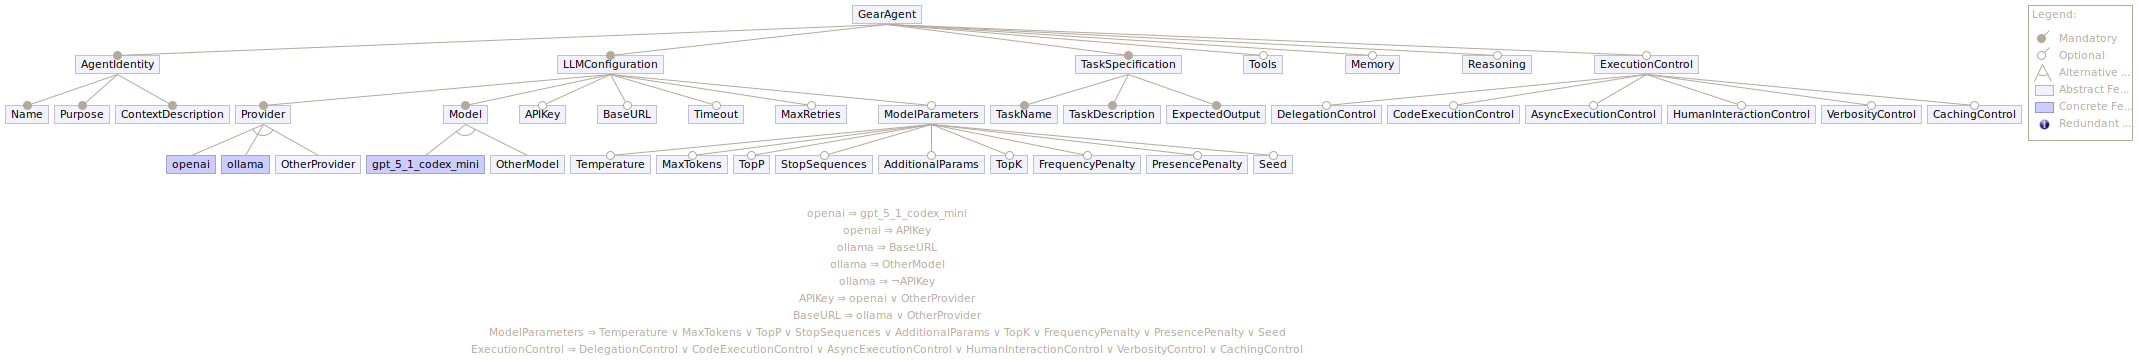
\includegraphics[width=\textwidth]
    {Figures/agent.png}

    \vspace{0.5em}

    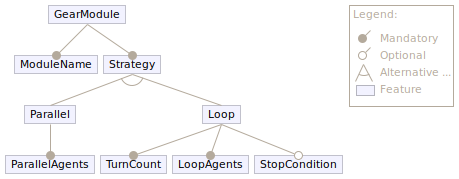
\includegraphics[width=0.48\textwidth]
    {Figures/module.png}
    \hfill
    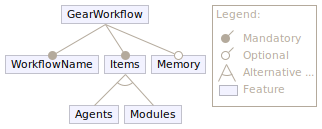
\includegraphics[width=0.48\textwidth]
    {Figures/workflow.png}

    \caption{GEAR feature models: \texttt{GearAgent} (top),
    \texttt{GearModule} (bottom left), and \texttt{GearWorkflow}
    (bottom right).}
    \label{fig:gear-feature-models}
\end{figure*}


\paragraph{\textbf{Definition and verification of constraints.}}
The features were connected through mandatory, optional, and alternative
relations. Mandatory relations represent elements required to define a valid
instance of their parent, while optional relations represent capabilities that
may be enabled depending on the intended system. Alternative groups represent
mutually exclusive configuration choices.

Cross-tree constraints were added when the hierarchy alone could not express a
dependency. For example, selecting the OpenAI provider requires an API key,
whereas selecting Ollama requires a base URL and excludes the OpenAI API key.
Similarly, selecting model parameters or execution controls requires at least
one corresponding subfeature.

The models and their constraints were expressed in the Universal Variability
Language (UVL). Framework-specific mechanisms that could not be generalized
were left to the mappings and connectors presented in the next subsection.

The resulting feature models constitute the common variability representation
used by GEAR. They separate the framework-independent specification of an
agentic system from the mechanisms required to instantiate it in a target
framework.

\subsection{Definition of Framework-Specific Mappings}
\label{subsec:mapping-target-frameworks}

The common variability model describes agents, modules, and workflows
independently of a particular framework. However, frameworks expose these
concepts through different APIs, properties, and execution mechanisms. A common
configuration decision may therefore have a direct representation in one
framework, require an adaptation in another, or remain unsupported.

GEAR addresses these differences through explicit mappings between the common
model and each supported target framework. These mappings separate the
description of the agentic system from the technical mechanisms used to
implement it.


\paragraph{\textbf{Identification of correspondences.}}
For each target framework, we examined how the concepts represented in
\texttt{GearAgent}, \texttt{GearModule}, and \texttt{GearWorkflow} can be
implemented using its public abstractions. At the agent level, this analysis
covered identity, models, instructions, tasks, tools, memory, reasoning, and
execution controls. At the module and workflow levels, it covered agent
composition, parallel and iterative execution, dependencies, and shared memory.

This step differs from the analysis performed during the derivation of the
common model. The previous step identified configuration concepts that are
relevant across frameworks. The present step determines how each concept can be
represented in a specific target framework.

For example, a parallel module may be implemented through a native parallel
agent, concurrent graph branches, or asynchronous execution primitives. These
mechanisms differ across frameworks but can represent the same orchestration
decision when they preserve the concurrent execution of the configured
elements.


\paragraph{\textbf{Definition of declarative mappings.}}
The identified correspondences were encoded in declarative YAML files. Separate
mappings describe agent, module, and workflow properties. Each entry identifies
a property from the common representation, its target abstraction, and the
nature of their correspondence.

A mapping entry follows the general structure:

\begin{verbatim}
- from: AgentIdentity.Name
  to: Agent.Name
  kind: direct
\end{verbatim}

The \texttt{from} field refers to a property in the common GEAR representation,
while the \texttt{to} field identifies its representation in the target
framework. Table~\ref{tab:mapping-types} presents the four correspondence types
used by GEAR.

\begin{table}[t]
    \centering
    \caption{Correspondence types used in framework mappings.}
    \label{tab:mapping-types}
    \footnotesize
    \begin{tabularx}{\columnwidth}{
        @{}
        p{0.23\columnwidth}
        >{\raggedright\arraybackslash}X
        @{}
    }
        \toprule
        \textbf{Type}
        & \textbf{Meaning} \\
        \midrule

        \texttt{direct}
        & The value can be transferred to a target property without changing
        its semantics. \\

        \texttt{equivalent}
        & The target uses a different abstraction that preserves the intended
        semantics. \\

        \texttt{partial}
        & The target represents only part of the common property or requires
        an explicit adaptation. \\

        \texttt{not\_mapped}
        & No sufficiently faithful target representation is available. \\

        \bottomrule
    \end{tabularx}
\end{table}

These mappings remain separate from the code-generation logic. They make the
correspondences inspectable and allow the support for a framework to evolve
without duplicating or modifying the common variability model.


\paragraph{\textbf{Treatment of semantic differences.}}
A valid GEAR configuration is not necessarily fully supported by every target
framework. When a framework provides a compatible abstraction, the selected
property is transferred directly or through an equivalent representation. When
only part of its semantics can be preserved, the mapping is declared as partial
and the required adaptation is handled during generation.

For example, a loop module may define both a maximum number of iterations and a
natural-language stopping condition. A target framework may support the
iteration limit without providing an executable representation of the stopping
condition. In this case, GEAR can map the iteration limit while explicitly
identifying the stopping condition as partially supported or unmapped.

The same issue occurs when a common property does not contain enough information
to construct the corresponding target element. A tool name, for instance, may
be insufficient when the framework also requires a callable implementation,
input schema, or dependency. GEAR does not generate such missing information
implicitly.

These distinctions prevent an incomplete translation from being considered
semantically exact. They also preserve traceability between the selected
features and their representation in the target framework. The mappings
therefore define the boundary between the common variability model and the
framework-specific generation mechanisms presented in
Section~\ref{subsec:gear-architecture-generation}.

\subsection{Iterative Validation and Refinement}
\label{subsec:iterative-validation-refinement}

The feature models, constraints, and framework-specific mappings were validated
iteratively against the artifacts of the ten selected frameworks. Missing
domain concepts were added, features were refined when their scope was too
general, and constraints were introduced when the comparison revealed
additional dependencies or incompatible choices.

The mappings were refined in the same loop. Implementing and exercising a
connector could reveal that a presumed direct correspondence required an
adaptation, that a target abstraction preserved only part of the intended
semantics, or that additional configuration information was required. The
correspondence type and the associated diagnostics were then updated
accordingly.

The process stopped when the common models covered the retained domain
concepts, their constraints admitted only structurally valid configurations,
and each selected feature had an explicit direct, equivalent, partial, or
unmapped status for every target framework. This iterative procedure separates
the construction and validation of the common representation from the tool
architecture that operationalizes it.

\section{The GEAR Tool}
\label{sec:gear-tool}
\label{subsec:gear-architecture-generation}

\subsection{Tool Overview and User Workflow}
\label{subsec:tool-overview-workflow}

GEAR implements the variability models and framework mappings through a
connector-based generation architecture. Its core components remain independent
of the target frameworks, while connectors encapsulate the information and
generation mechanisms required by each framework.

This separation enables the same GEAR configuration to be processed for
different targets without modifying the common variability model. It also
isolates framework-specific dependencies, templates, and adaptations from the
rest of the generation process.

From a user perspective, a GEAR workflow starts with the configuration of
agents, reusable modules, and their top-level composition. The user then selects
a target framework and requests generation. GEAR validates the configuration,
applies the corresponding mappings, produces the target project, and returns
the generated artifacts together with a conversion report.

\subsection{Tool Architecture}
\label{subsec:tool-architecture}

\paragraph{\textbf{Architecture overview.}}
Figure~\ref{fig:gear-architecture} presents the architecture of GEAR. The
configuration layer exposes the features defined by \texttt{GearAgent},
\texttt{GearModule}, and \texttt{GearWorkflow}. A selected configuration is
validated against these models before being transferred to the generation core.

The generation core interprets the selected features and constructs a
framework-independent intermediate representation of the configured system.
This representation describes the agents, modules, workflow structure,
properties, and relationships required for generation without relying on the
classes or syntax of a particular framework.

The connector corresponding to the selected target framework then translates
this representation into executable artifacts. It uses the mappings introduced
in Section~\ref{subsec:mapping-target-frameworks}, together with
framework-specific templates and assembly logic.

\begin{figure*}[t]
    \centering
    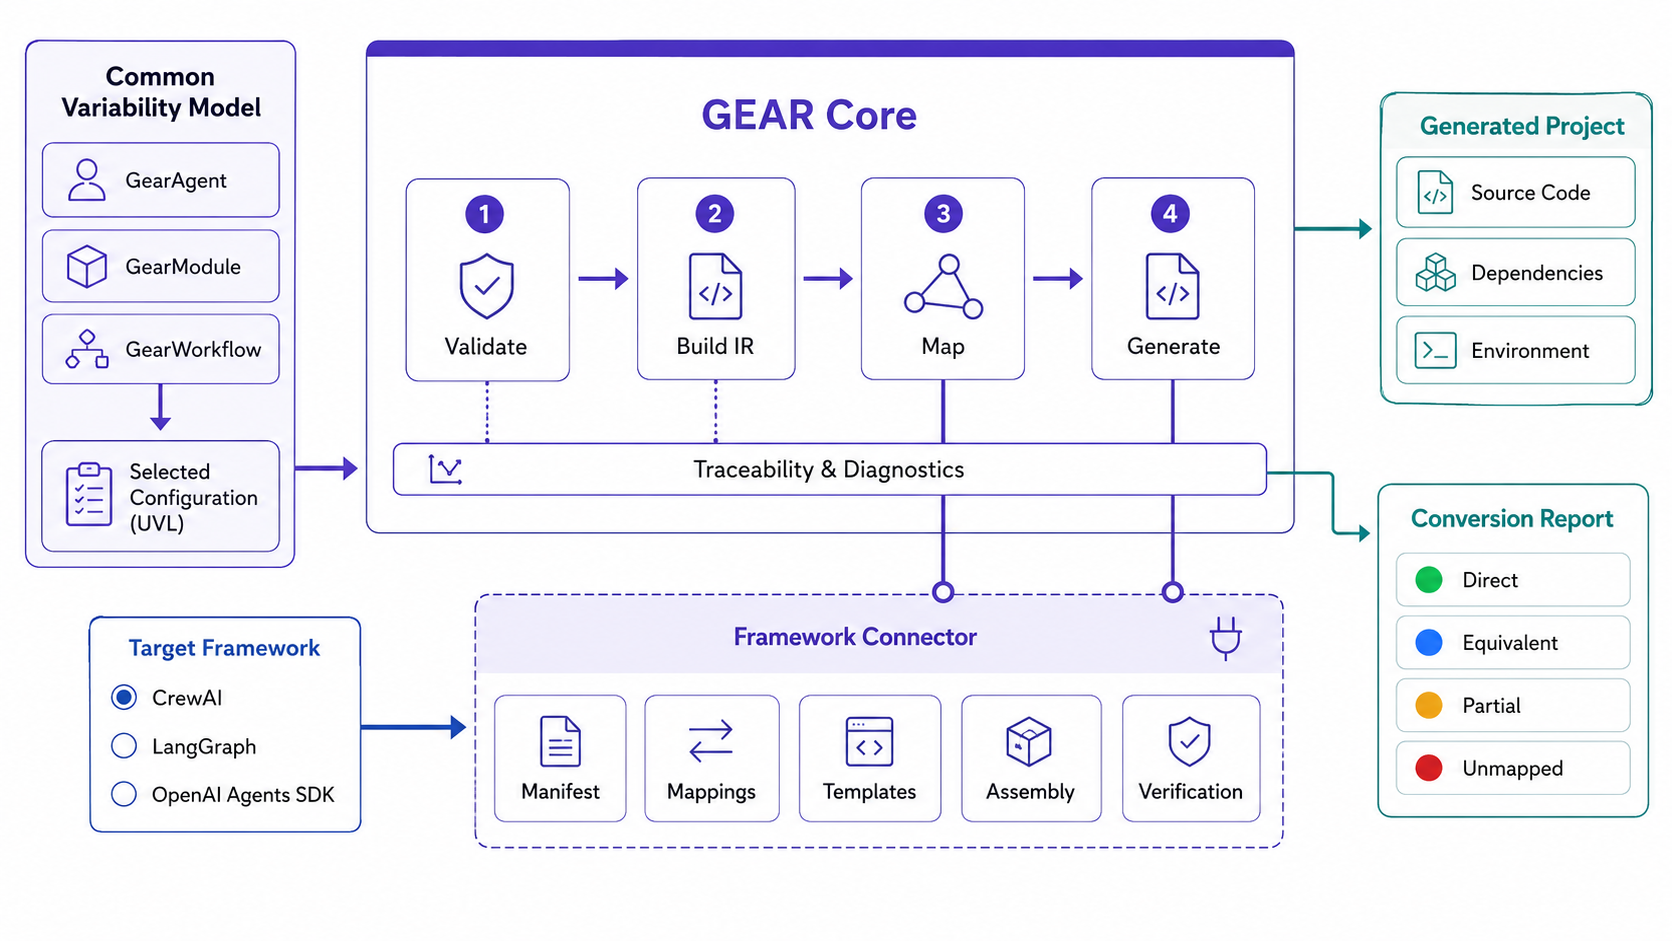
\includegraphics[width=\textwidth]
    {Figures/gear-architecture.png}
    \caption{Architecture and generation workflow of GEAR.}
    \label{fig:gear-architecture}
\end{figure*}


\paragraph{\textbf{Connector organization.}}
Each connector packages the resources required to support a target framework.
Table~\ref{tab:connector-components} summarizes its principal components.

\begin{table*}[t]
    \centering
    \caption{Principal components of a GEAR framework connector.}
    \label{tab:connector-components}
    \footnotesize
    \begin{tabularx}{\textwidth}{
        @{}
        p{0.20\textwidth}
        >{\raggedright\arraybackslash}X
        p{0.27\textwidth}
        @{}
    }
        \toprule
        \textbf{Component}
        & \textbf{Responsibility}
        & \textbf{Produced or consumed information} \\
        \midrule

        Manifest
        & Declares the connector, its target framework, supported artifacts,
        dependencies, and entry points
        & Connector metadata and compatibility information \\

        Mapping files
        & Associate properties of the common representation with
        target-framework abstractions
        & Direct, equivalent, partial, and unmapped correspondences \\

        Templates
        & Define the structure of the generated source files and configuration
        artifacts
        & Source code, dependency files, and environment templates \\

        Assembly plugin
        & Applies framework-specific transformations that cannot be expressed
        through declarative mappings alone
        & Imports, constructors, workflow composition, and execution logic \\

        Verification rules
        & Check target-specific requirements and unsupported combinations
        & Errors, warnings, and compatibility information \\

        \bottomrule
    \end{tabularx}
\end{table*}

The manifest provides the generation core with the information necessary to
load the connector. Mapping files handle correspondences that can be expressed
declaratively. Templates define the structure of the generated artifacts,
whereas the assembly plugin implements transformations that require executable
logic, such as constructing framework objects, connecting graph nodes,
registering tools, or assembling an execution entry point.

This organization avoids embedding framework-specific conditions directly into
the common generation core. A connector may therefore evolve independently when
the API of its target framework changes.


\paragraph{\textbf{Intermediate representation.}}
After validation, GEAR converts the selected features into an intermediate
representation organized around agents, modules, and workflows. Each element
contains its selected properties and references to related elements.

For example, an agent representation may contain its identifier, instructions,
model configuration, task, tools, memory options, and execution controls. A
module representation records its orchestration type, contained elements, and
optional aggregation or stopping configuration. The workflow representation
defines the top-level composition and shared resources.

The intermediate representation also preserves the origin of each property in
the variability model. This traceability allows GEAR to associate generated
elements and conversion diagnostics with the features selected by the user.

\subsection{Configuration Facilities}
\label{subsec:configuration-facilities}

GEAR exposes separate configuration facilities for individual agents, reusable
orchestration modules, and complete workflows. Agent configurations cover
identity, instructions, model parameters, tasks, tools, memory, outputs, and
execution controls. Module configurations capture parallel or iterative
composition, optional aggregation, and stopping conditions. Workflow
configurations assemble agents and modules, declare their dependencies, and
optionally define shared resources.

These facilities are driven by the \texttt{GearAgent},
\texttt{GearModule}, and \texttt{GearWorkflow} feature models. Consequently,
the available choices and their constraints are obtained from the common
variability representation rather than hard-coded for a target framework. The
target selection activates the relevant connector and its compatibility rules
without changing the source configuration.

\subsection{Code Generation and Validation}
\label{subsec:code-generation-validation}

\paragraph{\textbf{Generation workflow.}}
The generation process follows six steps:

\begin{enumerate}
    \item GEAR loads the configurations of the agents, modules, and workflow.

    \item The configurations are validated against their respective feature
    models and cross-tree constraints.

    \item The selected features are normalized into the framework-independent
    intermediate representation.

    \item The mapping files of the selected connector are applied to identify
    the corresponding target abstractions and their level of support.

    \item The connector combines the mapped properties, templates, and assembly
    logic to generate the source code and supporting artifacts.

    \item The generated project and the mapping results are verified before the
    project is returned to the user.
\end{enumerate}

The generated artifacts may include agent definitions, workflow construction
code, an execution entry point, dependency declarations, environment templates,
and framework-specific configuration files. The exact structure depends on the
target connector, while the configured system remains derived from the same
common representation.


\paragraph{\textbf{Verification and conversion report.}}
GEAR performs verification at both the common-model and target-framework
levels. Feature-model validation ensures that the selected configuration
satisfies the structural relations and cross-tree constraints defined in UVL.
Connector-level verification checks whether the mapped values satisfy the
requirements of the target framework.

The result of the conversion is documented in a report that distinguishes
properties mapped directly, represented through an equivalent abstraction,
partially supported, or left unmapped. The report also identifies missing
values, target-specific requirements, and adaptations performed by the
connector.

Consequently, successful code generation does not imply that every selected
property has been translated with identical semantics. The conversion report
makes such differences explicit and prevents partial support from being
presented as complete equivalence.

\subsection{Extending GEAR}
\label{subsec:extending-gear}

Support for a new framework is introduced by creating a connector containing
its manifest, mappings, templates, assembly logic, and verification rules. The
common variability model does not need to be modified when the new framework
provides alternative implementations of concepts already represented by GEAR.

An extension of the common model is required only when the framework introduces
a configuration decision that is relevant beyond its internal API and cannot be
expressed by the existing features. In this case, the new concept must first be
evaluated using the derivation process described in
Section~\ref{subsec:common-variability-model}. Its mappings can then be defined
for the frameworks able to represent it.

This architecture therefore separates three concerns: the definition of the
configuration space through the feature models, the semantic correspondences
expressed through mappings, and the technical generation mechanisms implemented
by the connectors.

\subsection{Implementation and Availability}
\label{subsec:implementation-availability}

GEAR is implemented as an open-source tool whose framework-independent assets
and target-specific assets remain physically separated. The common feature
models are represented in UVL, correspondence rules are stored in YAML mapping
files, and each connector packages its manifest, templates, assembly plugin,
and verification rules. This organization makes the models and mappings
inspectable independently of the generated source code.

The source code, feature models, connectors, and paper artifacts are available
in the public GEAR repository referenced in Section~\ref{data}. The repository
also provides the material required to reproduce the configurations and
framework translations used in this study, while the accompanying demonstration
video illustrates the end-to-end configuration and generation workflow.

\section{Evaluation Methodology}
\label{sec:evaluation-methodology}

\subsection{Evaluation Scope}
\label{subsec:evaluation-scope}

The evaluation of GEAR is organized around three complementary dimensions:
representational coverage and transformation fidelity, execution correctness and
behavioral fidelity, and usability and practical utility. The present evaluation
focuses on the first two dimensions. The third dimension will be investigated
separately through a participant-based study.

The first dimension evaluates the ability of GEAR to represent and preserve the
main design and orchestration capabilities of heterogeneous frameworks for
\gls{llm}-based \gls{mas}s. This dimension is examined in two directions. The
framework-to-GEAR direction determines whether the capabilities identified in the
ten selected frameworks can be expressed through the common variability model,
composed of \texttt{GearAgent}, \texttt{GearModule}, and
\texttt{GearWorkflow}. Conversely, the GEAR-to-framework direction determines
whether the properties expressed in a GEAR specification are preserved when they
are transformed into framework-specific implementations. This analysis considers
the mappings, transformations, and generated artefacts associated with each of the
ten frameworks presented in Table~\ref{tab:framework-metadata}.

The second dimension evaluates the generated artefacts at both the technical and
behavioral levels. Technical correctness concerns whether the generated artefacts
are syntactically valid, importable, and executable in their target frameworks.
Behavioral fidelity concerns whether their execution respects the orchestration
constraints expressed in the source GEAR specification, such as task ordering,
dependencies, parallel branches, synchronization points, conditional transitions,
and bounded loops. Controlled agent responses are used to isolate orchestration
behavior from the non-determinism of the underlying \gls{llm}s.

Cross-framework portability is examined across these two dimensions. The same
GEAR specifications are used as inputs for the different framework targets without
introducing framework-specific modifications into the source configurations. This
makes it possible to determine which properties are preserved across frameworks,
which require framework-specific adaptations, and which cannot be supported by a
given target. Unsupported or inapplicable capabilities remain part of the
evaluation and are reported explicitly rather than being excluded from the
analysis.

Table~\ref{tab:evaluation-scope} summarizes the dimensions considered, their
evaluation subjects, and the main forms of evidence used.

\begin{table*}[t]
    \centering
    \caption{Scope of the GEAR evaluation.}
    \label{tab:evaluation-scope}
    \footnotesize
    \begin{tabularx}{\textwidth}{
        @{}
        p{0.20\textwidth}
        p{0.26\textwidth}
        p{0.19\textwidth}
        >{\raggedright\arraybackslash}X
        @{}
    }
        \toprule
        \textbf{Dimension}
        & \textbf{Evaluated aspect}
        & \textbf{Subjects}
        & \textbf{Main evidence} \\
        \midrule

        Representational coverage
        & Framework capabilities expressible through the common variability model
        & Ten selected frameworks
        & Framework documentation, normalized capabilities, and GEAR features \\

        Transformation fidelity
        & Preservation of GEAR properties in framework-specific artefacts
        & Ten selected frameworks
        & Mappings, transformation reports, and generated source code \\

        Execution correctness
        & Syntactic validity, importability, and executability of generated artefacts
        & Generated implementations
        & Validation, import, and execution results \\

        Behavioral fidelity
        & Conformance of runtime behavior to the source GEAR specification
        & Generated workflow implementations
        & Expected and observed execution traces \\

        Usability and practical utility
        & Effort, understanding, and perceived usefulness
        & Future study participants
        & Task measurements, observations, and participant feedback \\

        \bottomrule
    \end{tabularx}
\end{table*}

The evaluation covers capabilities related to agent definition, configuration,
composition, orchestration, transformation, generation, and execution. It does not
assess the quality of the textual responses produced by the underlying
\gls{llm}s, model accuracy, token consumption, execution performance, or graphical
user interfaces. These aspects fall outside the current objectives, which concern
the representation, transformation, and execution of multi-agent system
configurations.

Finally, the ten frameworks considered in the representational analysis also
contributed to the construction of the common variability model. Consequently,
this part of the evaluation measures the coverage of the construction corpus. It
does not, by itself, demonstrate that GEAR generalizes to frameworks that were not
considered during the model derivation.

\subsection{Representational Coverage and Transformation Fidelity}
\label{subsec:representation-transformation}

This first evaluation axis examines two complementary properties of GEAR.
First, it determines whether the common variability model can represent the
design, configuration, and orchestration capabilities provided by the ten
selected frameworks. Second, it determines whether the semantics expressed
through GEAR are preserved when framework-specific artefacts are generated.

These two directions are evaluated using two matrices: a feature-presence
matrix for the analysis from the frameworks to GEAR, and a
semantic-preservation matrix for the analysis from GEAR to the target
frameworks. The normalized feature catalogue, the GEAR feature models, and
the framework connectors are fixed before the assessment. Consequently, this
evaluation does not modify the common model in response to the observed
results.

\paragraph{Feature-presence matrix.}

The feature-presence matrix evaluates the representational coverage of GEAR.
It answers the following question: \emph{to what extent can the capabilities
provided by each framework be represented through the common variability
model of GEAR?}

Each row corresponds to a normalized capability from the feature catalogue.
The capabilities cover agent definition, model and tool configuration, task
composition, memory, data exchange, orchestration, and execution management.
The columns correspond to GEAR and the ten selected frameworks.

Each cell is assigned one of the following values:

\begin{itemize}
    \item \textbf{F} (\emph{fully present}) indicates that the technology
    provides a construct that represents the complete semantics of the
    capability;
    
    \item \textbf{P} (\emph{partially present}) indicates that only a
    restricted form of the capability is available or that some of its
    semantics cannot be expressed; and
    
    \item \textbf{--} (\emph{absent}) indicates that no corresponding
    construct is available.
\end{itemize}

The classification of the framework cells is based on the official
documentation, public APIs, and examples associated with the reference
versions reported in Table~\ref{tab:framework-metadata}. For GEAR, the
classification is based on the features and constraints defined in
\texttt{GearAgent}, \texttt{GearModule}, and \texttt{GearWorkflow}. The
presence of a similarly named class or function is not considered sufficient
unless the expected semantics can also be represented.

Table~\ref{tab:feature-presence-matrix} presents the compact
feature-presence matrix used in the article. The detailed matrix, containing
all the individual features and variants of the common model, is provided in
the replication package.

\begin{table*}[t]
    \centering
    \caption{Feature-presence matrix used to evaluate the representational
    coverage of GEAR.}
    \label{tab:feature-presence-matrix}
    \scriptsize
    \setlength{\tabcolsep}{2pt}
    \renewcommand{\arraystretch}{1.08}
    \begin{tabularx}{\textwidth}{
        @{}
        >{\raggedright\arraybackslash}X
        ccccccccccc
        @{}
    }
        \toprule
        \textbf{Normalized capability}
        & \textbf{GEAR}
        & \textbf{CrewAI}
        & \textbf{Google ADK}
        & \textbf{LangGraph}
        & \textbf{OpenAI SDK}
        & \textbf{Microsoft AF}
        & \textbf{Strands}
        & \textbf{PydanticAI}
        & \textbf{AutoGen}
        & \textbf{Semantic K.}
        & \textbf{Haystack} \\
        \midrule
        
        Agent instructions
        & ? & ? & ? & ? & ? & ? & ? & ? & ? & ? & ? \\

        Model configuration
        & ? & ? & ? & ? & ? & ? & ? & ? & ? & ? & ? \\

        Task definition
        & ? & ? & ? & ? & ? & ? & ? & ? & ? & ? & ? \\

        Task dependencies
        & ? & ? & ? & ? & ? & ? & ? & ? & ? & ? & ? \\

        Tool association
        & ? & ? & ? & ? & ? & ? & ? & ? & ? & ? & ? \\

        Individual memory
        & ? & ? & ? & ? & ? & ? & ? & ? & ? & ? & ? \\

        Shared memory
        & ? & ? & ? & ? & ? & ? & ? & ? & ? & ? & ? \\

        Structured outputs
        & ? & ? & ? & ? & ? & ? & ? & ? & ? & ? & ? \\

        Agent delegation
        & ? & ? & ? & ? & ? & ? & ? & ? & ? & ? & ? \\

        Sequential execution
        & ? & ? & ? & ? & ? & ? & ? & ? & ? & ? & ? \\

        Parallel execution
        & ? & ? & ? & ? & ? & ? & ? & ? & ? & ? & ? \\

        Fan-out/fan-in
        & ? & ? & ? & ? & ? & ? & ? & ? & ? & ? & ? \\

        Conditional routing
        & ? & ? & ? & ? & ? & ? & ? & ? & ? & ? & ? \\

        Bounded loops
        & ? & ? & ? & ? & ? & ? & ? & ? & ? & ? & ? \\

        Asynchronous execution
        & ? & ? & ? & ? & ? & ? & ? & ? & ? & ? & ? \\

        Execution tracing
        & ? & ? & ? & ? & ? & ? & ? & ? & ? & ? & ? \\

        \bottomrule
    \end{tabularx}

    \vspace{0.3em}
        \begin{minipage}{0.98\textwidth}
            \scriptsize
            Cell values: F = fully present; P = partially present;
            -- = absent. OpenAI SDK denotes the OpenAI Agents SDK,
            and Microsoft AF denotes the Microsoft Agent Framework.
        \end{minipage}
\end{table*}

For a framework \(j\), let \(F^{*}_{j}\) denote the set of capabilities
provided by that framework and included in the functional scope of the
evaluation. Let \(R_{G,j}\) denote the subset of these capabilities that can
be represented, either fully or partially, by GEAR. The representational
coverage of GEAR for framework \(j\) is defined as:

\begin{equation}
    C_{\mathrm{repr}}(j)
    =
    \frac{|R_{G,j}|}{|F^{*}_{j}|}.
    \label{eq:representational-coverage}
\end{equation}

In addition to this overall value, the numbers of fully and partially
represented capabilities are reported separately. This distinction prevents
a partial representation from being interpreted as equivalent to a complete
one. The measure is calculated for each of the ten frameworks and aggregated
over the complete catalogue.

\paragraph{Semantic-preservation matrix.}

The semantic-preservation matrix evaluates the inverse direction, from GEAR
to the target frameworks. It answers the following question: \emph{to what
extent are the features and constraints expressed in a GEAR specification
preserved in the generated framework-specific artefacts?}

Each row corresponds to a configurable GEAR capability or constraint. When
the same capability has variants with different semantics, such as sequential
and parallel execution, these variants are represented by separate entries.
Each column corresponds to one of the ten target frameworks.

The same predefined GEAR specifications are transformed for the different
targets. No framework-specific modification is introduced into the source
configurations. This makes it possible to evaluate whether portability is
provided by the GEAR connectors rather than by manually adapting the source
specification for each framework.

Each cell of the semantic-preservation matrix is assigned one of the
following values:

\begin{itemize}
    \item \textbf{N} (\emph{native}) indicates that the target framework
    directly provides a construct that preserves the complete semantics of
    the GEAR capability;

    \item \textbf{S} (\emph{synthesized}) indicates that the connector
    generates additional code to reproduce the complete semantics of the
    capability;

    \item \textbf{A} (\emph{adapted}) indicates that the generated artefact
    supports the capability with a documented restriction or semantic
    difference;

    \item \textbf{U} (\emph{unsupported}) indicates that the connector cannot
    produce an implementation preserving the intended semantics; and

    \item \textbf{NA} (\emph{not applicable}) indicates that the capability
    is outside the execution model or functional scope of the target.
\end{itemize}

Native and synthesized transformations are both considered fully preserving.
The distinction describes the implementation mechanism, not its fidelity.
Conversely, an adapted transformation remains distinguishable because an
observable restriction or semantic difference is introduced.

Table~\ref{tab:semantic-preservation-matrix} presents the compact
semantic-preservation matrix. The complete matrix in the replication package
records the individual GEAR features, their variants, the corresponding
target constructs, and the evidence supporting each classification.

\begin{table*}[t]
    \centering
    \caption{Semantic-preservation matrix used to evaluate the transformation
    of GEAR features into framework-specific artefacts.}
    \label{tab:semantic-preservation-matrix}
    \scriptsize
    \setlength{\tabcolsep}{2pt}
    \renewcommand{\arraystretch}{1.08}
    \begin{tabularx}{\textwidth}{
        @{}
        >{\raggedright\arraybackslash}X
        cccccccccc
        @{}
    }
        \toprule
        \textbf{GEAR capability}
        & \textbf{CrewAI}
        & \textbf{Google ADK}
        & \textbf{LangGraph}
        & \textbf{OpenAI SDK}
        & \textbf{Microsoft AF}
        & \textbf{Strands}
        & \textbf{PydanticAI}
        & \textbf{AutoGen}
        & \textbf{Semantic Kernel}
        & \textbf{Haystack} \\
        \midrule

        Agent instructions
        & ? & ? & ? & ? & ? & ? & ? & ? & ? & ? \\

        Model configuration
        & ? & ? & ? & ? & ? & ? & ? & ? & ? & ? \\

        Task definition
        & ? & ? & ? & ? & ? & ? & ? & ? & ? & ? \\

        Task dependencies
        & ? & ? & ? & ? & ? & ? & ? & ? & ? & ? \\

        Tool association
        & ? & ? & ? & ? & ? & ? & ? & ? & ? & ? \\

        Individual memory
        & ? & ? & ? & ? & ? & ? & ? & ? & ? & ? \\

        Shared memory
        & ? & ? & ? & ? & ? & ? & ? & ? & ? & ? \\

        Structured outputs
        & ? & ? & ? & ? & ? & ? & ? & ? & ? & ? \\

        Agent delegation
        & ? & ? & ? & ? & ? & ? & ? & ? & ? & ? \\

        Sequential execution
        & ? & ? & ? & ? & ? & ? & ? & ? & ? & ? \\

        Parallel execution
        & ? & ? & ? & ? & ? & ? & ? & ? & ? & ? \\

        Fan-out/fan-in
        & ? & ? & ? & ? & ? & ? & ? & ? & ? & ? \\

        Conditional routing
        & ? & ? & ? & ? & ? & ? & ? & ? & ? & ? \\

        Bounded loops
        & ? & ? & ? & ? & ? & ? & ? & ? & ? & ? \\

        Natural-language stop condition
        & ? & ? & ? & ? & ? & ? & ? & ? & ? & ? \\

        Asynchronous execution
        & ? & ? & ? & ? & ? & ? & ? & ? & ? & ? \\

        Execution tracing
        & ? & ? & ? & ? & ? & ? & ? & ? & ? & ? \\

        \bottomrule
    \end{tabularx}

    \vspace{0.3em}
        \begin{minipage}{0.98\textwidth}
            \scriptsize
            Cell values: N = native; S = synthesized; A = adapted;
            U = unsupported; NA = not applicable. OpenAI SDK denotes
            the OpenAI Agents SDK, and Microsoft AF denotes the
            Microsoft Agent Framework.
        \end{minipage}
\end{table*}

For a target framework \(j\), let \(n_{N,j}\), \(n_{S,j}\),
\(n_{A,j}\), and \(n_{U,j}\) denote the numbers of native, synthesized,
adapted, and unsupported transformations, respectively. Entries classified
as not applicable are excluded from the calculations. The number of
applicable transformations is therefore:

\begin{equation}
    n_{\mathrm{app},j}
    =
    n_{N,j}
    +
    n_{S,j}
    +
    n_{A,j}
    +
    n_{U,j}.
    \label{eq:applicable-transformations}
\end{equation}

The semantic-preservation coverage measures the proportion of GEAR
capabilities whose complete semantics are preserved, either through a native
construct or through synthesized code:

\begin{equation}
    C_{\mathrm{pres}}(j)
    =
    \frac{n_{N,j}+n_{S,j}}
         {n_{\mathrm{app},j}}.
    \label{eq:preservation-coverage}
\end{equation}

Adapted capabilities are not included in this measure because their
transformation introduces a documented semantic difference. They are
reported separately through the adapted coverage:

\begin{equation}
    C_{\mathrm{adapt}}(j)
    =
    \frac{n_{A,j}}
         {n_{\mathrm{app},j}}.
    \label{eq:adapted-coverage}
\end{equation}

The unsupported coverage measures the proportion of applicable GEAR
capabilities for which no valid transformation is available:

\begin{equation}
    C_{\mathrm{unsupported}}(j)
    =
    \frac{n_{U,j}}
         {n_{\mathrm{app},j}}.
    \label{eq:unsupported-coverage}
\end{equation}

These three measures provide a complete decomposition of the applicable
transformations:

\begin{equation}
    C_{\mathrm{pres}}(j)
    +
    C_{\mathrm{adapt}}(j)
    +
    C_{\mathrm{unsupported}}(j)
    =
    1.
    \label{eq:transformation-decomposition}
\end{equation}

Because a transformation limitation must not remain silent, the assessment
also examines whether GEAR reports an explicit diagnostic for adapted and
unsupported capabilities. Let \(n_{\mathrm{diag},j}\) denote the number of
adapted or unsupported transformations for which the connector produces an
explicit diagnostic. Diagnostic coverage is defined as:

\begin{equation}
    C_{\mathrm{diag}}(j)
    =
    \frac{n_{\mathrm{diag},j}}
         {n_{A,j}+n_{U,j}}.
    \label{eq:diagnostic-coverage}
\end{equation}

When no adapted or unsupported capability is observed for a framework,
diagnostic coverage is reported as not applicable. The measures are reported
separately for each framework. Macro-aggregated results give the same weight
to each framework, whereas micro-aggregated results are computed from all
applicable matrix entries.

\paragraph{Evidence and traceability.}

Each classification is associated with evidence identifying the normalized
capability or GEAR feature, the corresponding framework construct, the
applicable documentation or API entry, the connector mapping, and the
generated source-code fragment. This information is stored in the
replication package together with the complete matrices and the scripts used
to calculate the reported measures.

The two matrices provide complementary evidence. The feature-presence matrix
determines whether the abstraction offered by GEAR covers the capabilities
available in the selected frameworks. The semantic-preservation matrix
determines how these abstractions are translated back into concrete
framework-specific implementations.

This analysis remains static: it establishes whether the required
information and semantics are represented in the common model and in the
generated source code. The following subsection evaluates whether the
generated artefacts are syntactically valid and executable, and whether
transformations classified as native, synthesized, or adapted are confirmed
by their observed runtime behavior.

\subsection{Execution Correctness and Behavioral Fidelity}
\label{subsec:execution-behavior}

This evaluation axis determines whether the framework-specific artefacts generated
by GEAR can be executed and whether their runtime behavior conforms to the source
GEAR specifications. While the previous analysis examines mappings and generated
code statically, this analysis provides dynamic evidence through validation,
execution, and trace comparison.

\paragraph{Execution correctness.}
Each evaluation specification is transformed into an implementation for every
applicable target framework. The generated artefacts are then assessed through
four successive stages:

\begin{enumerate}
    \item \emph{syntactic validation}, which checks that the generated source files
    can be parsed or compiled;
    \item \emph{dependency and import validation}, which checks that the generated
    project can load the required framework components;
    \item \emph{initialization validation}, which checks that the agents, tasks,
    modules, and workflows can be instantiated; and
    \item \emph{execution validation}, which checks that the generated workflow can
    run to completion without an error attributable to the transformation.
\end{enumerate}

A generated implementation is considered executable only if it passes all four
stages. Failures are recorded with their stage, framework, specification, and
error message. When a GEAR property is unsupported by a target framework, the
expected behavior is an explicit diagnostic during validation or generation,
rather than the production of a silently incomplete implementation.

For a target framework \(t\), execution correctness is measured as:

\begin{equation}
    \mathrm{ExecRate}_t =
    \frac{N^{\mathrm{executed}}_t}
         {N^{\mathrm{applicable}}_t},
\end{equation}

where \(N^{\mathrm{applicable}}_t\) is the number of implementations expected to
be generated and executed for framework \(t\), and
\(N^{\mathrm{executed}}_t\) is the number that successfully pass all validation
and execution stages. Stage-specific success rates are also reported to
distinguish generation, import, initialization, and runtime failures.

\paragraph{Behavioral fidelity.}
Successful execution alone does not demonstrate that the generated implementation
preserves the workflow semantics. Behavioral fidelity is therefore evaluated by
comparing the observed execution trace with an expected trace derived from the
source GEAR specification.

The evaluation scenarios are constructed to exercise the orchestration constructs
defined by \texttt{GearWorkflow}, including sequential execution, dependencies,
parallel branches, synchronization points, conditional transitions, and bounded
loops. Where applicable, scenarios also exercise agent delegation and the
transmission of outputs between dependent tasks.

For each scenario, the source specification is converted into a set of observable
constraints. These constraints define, for example:

\begin{itemize}
    \item which tasks must be executed;
    \item which task must precede another;
    \item which tasks may execute concurrently;
    \item which branches may be activated under a given condition;
    \item where parallel branches must be synchronized;
    \item how many times a bounded loop must be executed; and
    \item which outputs must be made available to dependent tasks.
\end{itemize}

The generated implementations are instrumented using a common trace format. Each
event records at least the target framework, scenario, agent, task, event type,
and execution order. Framework-specific traces are normalized before comparison
so that differences in logging formats do not affect the assessment.

Controlled task outputs and deterministic conditions are used during execution.
This isolates orchestration behavior from the variability of the underlying
\gls{llm}s. Consequently, the evaluation concerns the behavior produced by the
generated orchestration logic and not the quality of the textual responses
generated by a model.

Let \(K_s\) denote the set of behavioral constraints derived from specification
\(s\), and let \(K^{\mathrm{sat}}_{s,t}\) denote the constraints satisfied by the
trace observed for target framework \(t\). Behavioral fidelity is measured as:

\begin{equation}
    \mathrm{TraceConformance}_{s,t} =
    \frac{|K^{\mathrm{sat}}_{s,t}|}{|K_s|}.
\end{equation}

A trace is considered fully conformant when all applicable constraints are
satisfied. Violations are reported individually and classified according to the
affected property, such as ordering, dependency, branching, synchronization,
iteration, or data transmission.

The same source specifications, controlled outputs, and trace constraints are
used across the target frameworks. This enables a cross-framework comparison
without introducing framework-specific changes into the GEAR configurations.
The execution results are also compared with the semantic preservation matrix.
A property classified as \emph{direct} or \emph{equivalent} is expected to
produce a conformant trace, whereas a \emph{partial} classification must exhibit
only the limitations declared during the static analysis. Any additional runtime
deviation is recorded as a discrepancy between the static mapping and the
observed behavior.
% \section{Evaluation Methodology}
\label{sec:evaluation-methodology}

This section presents the methodology used to evaluate the functional
coverage of GEAR. We first define the functional scope of the study from
dimensions identified in the scientific literature on \gls{llm}-based agents
and \gls{mas}. We then select a diverse set of general-purpose
frameworks through explicit eligibility and diversity criteria. Finally, the
retained characteristics and frameworks provide the basis for the
coverage analysis presented in the following subsections.

\subsection{Definition of the Functional Scope}
\label{subsec:functional-scope}

Before evaluating GEAR and the studied frameworks, we define the functional
scope of the study independently of the current capabilities of GEAR. This
separation prevents the evaluation scope from being restricted to features
already supported by the tool and, consequently, avoids artificially
increasing its measured coverage.

The candidate functional categories were identified through an analysis of
the scientific literature on \gls{llm}-based agents and \gls{mas}s.
Existing studies describe these systems through dimensions such as agent
profiles, goals, reasoning, planning, memory, action, tool use, perception,
environment interaction, communication, coordination, and capability
acquisition \cite{xi2025rise,guo2024large}. \etal{Wu}~\cite{wu2024autogen}
additionally emphasize configurable agents, human involvement, tool use, and
programmable interaction patterns. At the system level, topology,
orchestration logic, memory management, communication protocols, and
error-handling strategies can significantly influence the behaviour and
performance of a \gls{mas} \cite{emde2026maseval}. Finally,
\etal{Dong}~\cite{dong2024agentops} identify traces, logs, metrics, and runtime
artefacts as important elements for observing agentic systems.

These dimensions constitute the initial set of candidate characteristics. We
then selected those that correspond to the objective of this study: evaluating
the configuration, orchestration, and execution capabilities of
general-purpose frameworks for \gls{llm}-based \gls{mas}s. A
characteristic is included when it:

\begin{itemize}
    \item represents an explicit design or configuration decision;
    \item affects the structure, behaviour, or execution of the resulting
    \gls{mas};
    \item can be identified across multiple general-purpose frameworks; and
    \item can be evaluated independently of a particular application domain,
    model-training process, or deployment infrastructure.
\end{itemize}

Table~\ref{tab:functional-scope} reports the resulting functional scope. A
check mark indicates that a category is included in the study, whereas a cross
indicates that the category is scientifically relevant but outside the scope
of the present evaluation.

\begin{table}[t]
    \centering
    \caption{Functional categories identified from the literature and their
    inclusion in the scope of the study.}
    \label{tab:functional-scope}
    \footnotesize
    \begin{tabularx}{\textwidth}{
        @{}
        p{0.17\textwidth}
        >{\raggedright\arraybackslash}X
        >{\centering\arraybackslash}p{0.09\textwidth}
        p{0.29\textwidth}
        @{}
    }
        \toprule
        \textbf{Category}
        & \textbf{Considered characteristics}
        & \textbf{Included}
        & \textbf{Scope rationale} \\
        \midrule

        Agent specification
        & Identity, role, goals, instructions, capabilities, and contextual
        description
        & \included
        & These elements define the responsibilities and expected behaviour
        of each agent. \\

        Model configuration
        & Model, provider, endpoint, generation parameters, timeout, and retry
        parameters
        & \included
        & These configuration decisions can affect agent behaviour and
        execution across frameworks. \\

        Tasks and planning
        & Task descriptions, objectives, inputs, expected outputs,
        decomposition, and dependencies
        & \included
        & Tasks constitute configurable units of work and define how system
        objectives are operationalized. \\

        Tools
        & Tool declarations, tool schemas, association with agents, and tool
        invocation
        & \included
        & Tools determine how agents act on external resources and extend
        their capabilities. \\

        Memory and state
        & Individual memory, shared memory, workflow state, and propagation of
        intermediate results
        & \included
        & Memory and state determine how information is retained and shared
        during execution. \\

        Data and outputs
        & Textual outputs, JSON outputs, typed models, schemas, and output
        validation
        & \included
        & Output contracts determine how information is exchanged among
        tasks, agents, and external components. \\

        Orchestration and topology
        & Sequential and parallel execution, delegation, handoffs,
        fan-out/fan-in, aggregation, nodes, edges, and dependencies
        & \included
        & These characteristics define the structural organization and
        coordination of the system. \\

        Control flow
        & Conditions, branches, loops, routing decisions, and termination
        conditions
        & \included
        & Control-flow mechanisms determine which components are executed and
        under which conditions. \\

        Execution properties
        & Synchronous and asynchronous execution, execution limits, retries,
        error handling, caching, and human intervention
        & \included
        & These properties influence the runtime semantics and robustness of
        the resulting system. \\

        \midrule

        Communication protocols
        & Explicit messages, message types, communication channels,
        conversation protocols, and negotiation mechanisms
        & \excluded
        & Communication is a central multi-agent dimension, but comparing
        protocol semantics requires a separate interaction-level analysis. \\

        Perception and environment
        & Sensor modalities, perception pipelines, environment models, and
        environment-specific actions
        & \excluded
        & The study focuses on orchestrated software agents rather than
        embodied agents or domain-specific perception mechanisms. \\

        Learning and evolution
        & Online learning, self-improvement, capability acquisition, and
        runtime evolution
        & \excluded
        & The study evaluates system configuration and execution, not model
        training or agent-learning processes. \\

        Observability
        & Traces, logs, metrics, monitoring, runtime events, and execution
        analytics
        & \excluded
        & Observability concerns the operational analysis of executions and
        is assessed separately from functional coverage. \\

        Security and governance
        & Identities, permissions, access control, isolation, policy
        enforcement, and audit mechanisms
        & \excluded
        & These mechanisms require a dedicated security model, threat
        analysis, and evaluation protocol. \\

        \bottomrule
    \end{tabularx}
\end{table}

The retained scope therefore covers the declarative and executable
characteristics required to configure agents, assign tasks and tools, manage
memory and data, organize the system, control its execution flow, and define
its runtime properties. These characteristics are sufficiently general to be
examined across the studied frameworks while remaining directly related to
the configuration and execution concerns addressed by this study.

Some important dimensions identified in the literature are deliberately
excluded. In particular, communication is widely recognized as a central
property of \gls{mas}s
\cite{guo2024large,wu2024autogen,emde2026maseval}. However, the present study
does not compare message formats, communication languages, channels,
conversation protocols, or negotiation strategies. Handoffs, task
dependencies, shared state, and fan-out/fan-in structures remain included, but
they are examined as orchestration mechanisms rather than as communication
protocols.

Perception and environment modelling are excluded because the study focuses
on software agents operating through tasks, tools, and workflows rather than
on embodied agents or domain-specific sensing mechanisms. Learning and runtime
evolution are also excluded because the evaluation does not concern model
training, online learning, or agent self-improvement. Security and governance
would require a dedicated threat model and evaluation protocol and are
therefore left for future work.

Observability is handled separately. Although traces, logs, metrics, and
runtime artefacts are important for analysing agentic systems
\cite{dong2024agentops}, they describe how executions are monitored rather
than the functional configuration of a \gls{mas}. They are therefore
assessed in the operational evaluation rather than in the functional coverage
analysis.


\subsection{Selection of the Studied Frameworks}
\label{subsec:framework-selection}

After defining the functional scope, we selected the frameworks used to
conduct the coverage evaluation. The objective was not to establish an
exhaustive inventory or ranking of existing frameworks, but to construct a
diverse and reproducible sample covering different approaches to the design
and orchestration of \gls{llm}-based \gls{mas}s.

A framework was eligible for inclusion when it satisfied the following
criteria:

\begin{itemize}
    \item it was publicly accessible and sufficiently documented;
    \item it provided a Python API;
    \item it supported the definition of at least one \gls{llm}-based agent;
    \item it supported the composition of multiple agents, tasks, or workflow
    components;
    \item it provided an identifiable and installable version; and
    \item it was actively maintained at the time of selection.
\end{itemize}

Conversely, we excluded libraries limited to direct \gls{llm} calls, closed
platforms without an accessible API, inactive projects, frameworks exclusively
intended for reinforcement-learning agents, and observability tools that did
not support the construction of \gls{mas}s. Frameworks exclusively
targeting programming languages other than Python were also excluded.

Among the eligible frameworks, we adopted a purposive sampling strategy to
maximize the diversity of the sample. In particular, we sought complementary
approaches to agent specification, task definition, tool use, memory
management, orchestration, control flow, and execution. The selected
frameworks consequently represent systems organized around roles and tasks,
conversational teams, graph-based workflows, typed agent definitions,
pipeline-based architectures, and agent SDKs maintained by different
organizations. The frameworks were selected for this complementarity rather
than for their ability to cover every characteristic retained in the
functional scope; the absence of a characteristic from a framework is itself
an outcome of the subsequent coverage analysis.

The resulting sample comprises CrewAI, Google ADK, LangGraph, OpenAI Agents
SDK, Microsoft Agent Framework, Strands Agents, PydanticAI, AutoGen, Semantic
Kernel, and Haystack. Table~\ref{tab:selected-frameworks} presents the main
paradigm for which each framework was included. This classification indicates
the principal contribution of each framework to the diversity of the sample;
it does not imply that a framework is limited to a single paradigm.

\begin{table}[t]
    \centering
    \caption{Selected frameworks and their main represented paradigms.}
    \label{tab:selected-frameworks}
    \small
    \begin{tabularx}{\columnwidth}{
        @{}
        p{0.28\columnwidth}
        >{\raggedright\arraybackslash}X
        @{}
    }
        \toprule
        \textbf{Framework} & \textbf{Main represented paradigm} \\
        \midrule
        CrewAI
            & Role- and task-based agent organization \\
        Google ADK
            & Hierarchical agents and workflow agents \\
        LangGraph
            & Graph-based orchestration with state management \\
        OpenAI Agents SDK
            & Agents, agent handoffs, and tracing \\
        Microsoft Agent Framework
            & Enterprise workflows and fan-out/fan-in orchestration \\
        Strands Agents
            & Lightweight agent composition and agent graphs \\
        PydanticAI
            & Typed agents and structured outputs \\
        AutoGen
            & Agent conversations and teams \\
        Semantic Kernel
            & Agents, services, and enterprise plugins \\
        Haystack
            & Component pipelines and agent workflows \\
        \bottomrule
    \end{tabularx}
\end{table}

To support traceability and reproducibility, we fixed one reference version
for each framework. These versions correspond to the minimum versions
explicitly targeted by the GEAR connectors at the time of the study. For each
framework, we recorded the reference version, its release date, its official
documentation, and the reason for its inclusion.
Table~\ref{tab:framework-metadata} reports these metadata.

\begin{table*}[t]
    \centering
    \caption{Metadata documenting the selection of the studied frameworks.
    The versions correspond to the reference versions targeted by GEAR.}
    \label{tab:framework-metadata}
    \small
    \begin{tabular}{
        @{}
        p{0.18\textwidth}
        p{0.08\textwidth}
        p{0.10\textwidth}
        p{0.17\textwidth}
        p{0.32\textwidth}
        @{}
    }
        \toprule
        \textbf{Framework}
        & \textbf{Version}
        & \textbf{Release date}
        & \textbf{Official source}
        & \textbf{Reason for inclusion} \\
        \midrule

        CrewAI
        & 1.15.4
        & 2026-07-17
        & \href{https://docs.crewai.com/}{Documentation}
        & Role- and task-based orchestration \\

        Google ADK
        & 2.5.0
        & 2026-07-16
        & \href{https://adk.dev/}{Documentation}
        & Hierarchical agents and graph-based workflow agents \\

        LangGraph
        & 1.0.0
        & 2025-10-17
        & \href{https://docs.langchain.com/oss/python/langgraph/overview}
        {Documentation}
        & Stateful graph-based workflows with branching and joins \\

        OpenAI Agents SDK
        & 0.18.0
        & 2026-07-07
        & \href{https://openai.github.io/openai-agents-python/}
        {Documentation}
        & Agent handoffs and native tracing capabilities \\

        Microsoft Agent Framework
        & 1.11.0
        & 2026-07-10
        & \href{https://learn.microsoft.com/en-us/agent-framework/}
        {Documentation}
        & Enterprise agent workflows with fan-out and synchronized fan-in
        orchestration \\

        Strands Agents
        & 1.48.0
        & 2026-07-17
        & \href{https://strandsagents.com/docs/}
        {Documentation}
        & Lightweight composition of deterministic multi-agent graphs \\

        PydanticAI
        & 2.13.0
        & 2026-07-18
        & \href{https://pydantic.dev/docs/ai/overview/}
        {Documentation}
        & Type-safe agents and structured outputs \\

        AutoGen
        & 0.7.5
        & 2025-09-30
        & \href{https://microsoft.github.io/autogen/stable/user-guide/agentchat-user-guide/index.html}
        {Documentation}
        & Conversational agents and bounded agent teams \\

        Semantic Kernel
        & 1.44.0
        & 2026-07-07
        & \href{https://learn.microsoft.com/en-us/semantic-kernel/frameworks/agent/}
        {Documentation}
        & Service- and plugin-oriented agent architecture \\

        Haystack
        & 2.31.0
        & 2026-07-08
        & \href{https://docs.haystack.deepset.ai/docs/intro}
        {Documentation}
        & Pipeline-oriented agent and component composition \\

        \bottomrule
    \end{tabular}
\end{table*}

The functional scope defines the characteristics examined in the study,
whereas the selected frameworks define the systems against which GEAR is
evaluated. Together, these two elements provide the basis for the
bidirectional functional coverage analysis.
\subsection{Construction of the Feature Catalogue}
\label{subsec:feature-catalogue}

The functional scope defined in
Section~\ref{subsec:functional-scope} identifies the categories considered in
the evaluation. However, these categories remain too broad to support a
feature-level comparison between GEAR and the selected frameworks. We
therefore constructed a normalized feature catalogue that decomposes each
retained category into concrete and independently assessable features. This
catalogue constitutes the common reference used to build the coverage
matrices.

\subsubsection{Feature Identification}

Features were identified from two complementary sources. For GEAR, we examined
the metamodel, the feature models, the connector implementations, and the
generated code. For each studied framework, we examined the versioned official
documentation, API references, and implementation examples associated with
the version reported in Section~\ref{subsec:framework-selection}. When the
documentation was insufficient to determine the semantics of a construct, its
implementation or an executable example was additionally inspected.

Let $\mathcal{F}_{G}$ denote the set of features identified in GEAR and
$\mathcal{F}_{j}$ the set identified in framework $j$. Before filtering and
normalization, the initial set of candidate features is defined as:

\begin{equation}
    \mathcal{F}_{\mathrm{raw}}
    =
    \mathcal{F}_{G}
    \cup
    \bigcup_{j=1}^{m}\mathcal{F}_{j},
    \qquad m = 10.
    \label{eq:raw-feature-catalogue}
\end{equation}

This union ensures that the catalogue is not restricted to the features
currently represented by GEAR. A feature exposed by only one framework is
therefore retained as a candidate when it belongs to the functional scope of
the study.

The extraction focused on explicit constructs that allow developers to
configure the agents, models, tasks, tools, memory, data, orchestration,
control flow, or execution properties of a multi-agent system. Each candidate
was recorded together with its original terminology and the documentation,
API element, source file, or executable example from which it was identified.

\subsubsection{Scope-Based Filtering}

The candidate features were subsequently filtered according to the functional
scope established independently in
Section~\ref{subsec:functional-scope}. Let $\mathcal{C}^{*}$ denote the set of
functional categories included in the study and
$\operatorname{cat}(f)$ the category assigned to a candidate feature $f$. The
scope-filtered set is defined as:

\begin{equation}
    \mathcal{F}_{\mathrm{scope}}
    =
    \left\{
        f \in \mathcal{F}_{\mathrm{raw}}
        \;\middle|\;
        \operatorname{cat}(f) \in \mathcal{C}^{*}
    \right\}.
    \label{eq:scope-filtered-features}
\end{equation}

Consequently, the catalogue excludes constructs that do not concern the
functional configuration, orchestration, or execution of the studied
multi-agent systems. These include:

\begin{itemize}
    \item provider-specific deployment services and proprietary cloud
    capabilities;
    \item billing, account-management, and authentication mechanisms;
    \item framework-specific graphical interfaces;
    \item observability, monitoring, and execution-analytics services;
    \item security and governance mechanisms; and
    \item general-purpose data-processing capabilities that are not directly
    involved in the design or orchestration of agents.
\end{itemize}

These exclusions do not imply that the corresponding capabilities are
unimportant. They indicate that they belong to dimensions that require
different evaluation objectives and protocols. In particular, observability
is addressed separately in the operational evaluation and is therefore not
included in the functional coverage catalogue.

\subsubsection{Semantic Normalization}

The terminology used by the frameworks cannot be compared directly. Different
terms may refer to equivalent capabilities, while similar terms may conceal
different execution semantics. We therefore normalized the extracted features
according to their meaning rather than their names.

Two candidate features were merged when they represented the same
configuration decision and produced equivalent observable effects on the
structure or execution of the multi-agent system. Conversely, they were kept
separate when their differences affected at least one of the following
properties:

\begin{itemize}
    \item the entities involved, such as agents, tasks, tools, or workflow
    nodes;
    \item the direction and propagation of data;
    \item the ordering or concurrency of execution;
    \item the conditions governing branching, routing, or termination;
    \item the creation, persistence, or sharing of state;
    \item the aggregation of intermediate results; or
    \item execution constraints such as iteration limits, timeouts, retries,
    or human intervention.
\end{itemize}

For example, sequential execution and task dependency were retained as
distinct features. Sequential execution specifies an execution order, whereas
a dependency additionally expresses that one component relies on the
completion or result of another. Similarly, individual memory, shared memory,
and workflow state were not merged because they differ in ownership,
visibility, and lifetime.

Let $\sim_{\mathrm{sem}}$ denote the semantic equivalence relation established
through these criteria. The final normalized catalogue is the quotient set:

\begin{equation}
    \mathcal{F}^{*}
    =
    \mathcal{F}_{\mathrm{scope}}
    \big/
    {\sim_{\mathrm{sem}}}.
    \label{eq:normalized-feature-catalogue}
\end{equation}

Each equivalence class in $\mathcal{F}^{*}$ represents one normalized feature,
independently of the terminology used by GEAR or the individual frameworks.
This normalization avoids counting lexical variants as separate features
while preserving distinctions that may affect coverage or semantic fidelity.

\subsubsection{Catalogue Structure and Traceability}

Each normalized feature is documented through:

\begin{itemize}
    \item a unique identifier;
    \item its functional category;
    \item a framework-independent name and definition;
    \item the semantic criteria that must be satisfied for the feature to be
    considered covered;
    \item the technologies in which the feature was identified; and
    \item the corresponding evidence, including documentation references, API
    elements, source files, examples, or executable tests.
\end{itemize}

Table~\ref{tab:functional-catalogue-example} provides an illustrative excerpt
from this structure. The complete catalogue, including the provenance and
evidence associated with every feature, is provided in the replication
package.

\begin{table*}[t]
    \centering
    \caption{Illustrative structure of the normalized feature catalogue.}
    \label{tab:functional-catalogue-example}
    \footnotesize
    \begin{tabularx}{\textwidth}{
        @{}
        l
        p{0.15\textwidth}
        p{0.16\textwidth}
        >{\raggedright\arraybackslash}X
        p{0.27\textwidth}
        @{}
    }
        \toprule
        \textbf{ID}
        & \textbf{Category}
        & \textbf{Feature}
        & \textbf{Definition}
        & \textbf{Semantic criteria} \\
        \midrule

        AG1
        & Agent specification
        & Agent instructions
        & Definition of the behaviour expected from an agent
        & Instructions are explicitly associated with a specific agent and
        influence its behaviour. \\

        TK1
        & Tasks and planning
        & Task dependency
        & Requirement that one task be completed before another task can
        proceed
        & The dependency constrains execution and, when required, propagates
        the result of the preceding task. \\

        OR1
        & Orchestration and topology
        & Sequential execution
        & Execution of agents, tasks, or nodes according to a defined order
        & The order is preserved and a component starts only after its
        predecessor has completed. \\

        OR2
        & Orchestration and topology
        & Parallel execution
        & Concurrent execution of independent agents, tasks, or branches
        & Independent components may execute concurrently without an imposed
        sequential order. \\

        OR3
        & Orchestration and topology
        & Fan-in
        & Synchronization of results produced by multiple execution branches
        & Downstream execution waits for and combines the required upstream
        results. \\

        CT1
        & Control flow
        & Bounded loop
        & Repetition of an execution block subject to a maximum number of
        iterations
        & The loop may repeat a component while enforcing an explicit upper
        bound. \\

        \bottomrule
    \end{tabularx}
\end{table*}

The resulting catalogue defines the unit of analysis used throughout the
functional coverage evaluation. It supports the construction of two
complementary matrices: one determining which GEAR features can be generated
for each target framework, and another determining which framework features
can be represented by the GEAR metamodel. The construction and interpretation
of these matrices are presented in the following subsection.





\section*{Data Availability}
\label{data}
\texttt{GEAR} is open-source and available at \url{https://github.com/brellsanwouo/gear-framework}. 
A demonstration video presenting an end-to-end case study is also available at \url{https://youtu.be/K-V77HbWxv0}.The GitHub repository additionally   the complete visual representations of the \texttt{GEAR} feature models and the artifacts used in this paper.
\clearpage
\bibliographystyle{ACM-Reference-Format}
\bibliography{bibfile.bib}

\clearpage

\section*{appendix}

%\appendix

\section{Candidate Framework Identification and Screening}
\label{appendix:candidate-frameworks}

Table~\ref{tab:candidate-framework-screening} reports the frameworks identified
during the construction of the candidate pool. For each framework, it indicates
the source through which it was identified, the screening decision, and the
reason for its inclusion or exclusion, and its documentation. The initial
catalogue comprises the 22 entries supplied during framework identification.
The supplementary search added ten projects found through official
documentation and public repositories. Names were normalized when the
catalogue contained a typographical variant (e.g., ``Voltage'' for VoltAgent).
The screening information and documentation links were last verified in July
2026. A repository or package page is reported when a project does not provide
a separate documentation site.

\footnotesize
\setlength{\LTpre}{0.5\baselineskip}
\setlength{\LTpost}{0pt}
\begin{longtable}{
    @{}
    p{0.14\textwidth}
    p{0.13\textwidth}
    >{\centering\arraybackslash}p{0.10\textwidth}
    p{0.31\textwidth}
    p{0.18\textwidth}
    @{}
}
    \caption{Candidate frameworks, screening decisions, and documentation.}
    \label{tab:candidate-framework-screening} \\
    \toprule
    \textbf{Framework}
    & \textbf{Identification source}
    & \textbf{Decision}
    & \textbf{Reason}
    & \textbf{Documentation} \\
    \midrule
    \endfirsthead

    \multicolumn{5}{l}{\footnotesize
        \tablename~\thetable\ (continued)} \\
    \toprule
    \textbf{Framework}
    & \textbf{Identification source}
    & \textbf{Decision}
    & \textbf{Reason}
    & \textbf{Documentation} \\
    \midrule
    \endhead

    \midrule
    \multicolumn{5}{r}{\footnotesize Continued on next page} \\
    \endfoot

    \bottomrule
    \endlastfoot

    CrewAI
    & Initial catalogue
    & \cellcolor{green!25}Included
    & Meets all criteria; represents role- and task-based multi-agent
    orchestration.
    & \href{https://docs.crewai.com/}{Official docs} \\

    Google ADK
    & Initial catalogue
    & \cellcolor{green!25}Included
    & Meets all criteria; provides hierarchical agents and graph-based workflow
    agents.
    & \href{https://adk.dev/}{Official docs} \\

    Agno
    & Initial catalogue
    & Not selected
    & Eligible, but its team and workflow abstractions overlapped with the
    selected portfolio.
    & \href{https://docs.agno.com/}{Official docs} \\

    OpenAI Agents SDK
    & Initial catalogue
    & \cellcolor{green!25}Included
    & Meets all criteria; contributes handoffs, guardrails, sessions, and
    native tracing.
    & \href{https://openai.github.io/openai-agents-python/}{Official docs} \\

    Portia SDK
    & Initial catalogue
    & Not selected
    & Eligible Python SDK, but not retained after diversity-based selection.
    & \href{https://github.com/portiaAI/portia-sdk-python\#readme}
    {Repository docs} \\

    AutoGen
    & Initial catalogue
    & \cellcolor{green!25}Included
    & Meets all criteria; represents conversational agents and bounded agent
    teams.
    & \href{https://microsoft.github.io/autogen/stable/}{Official docs} \\

    LangGraph
    & Initial catalogue
    & \cellcolor{green!25}Included
    & Meets all criteria; represents stateful graph workflows with branches
    and joins.
    & \href{https://docs.langchain.com/oss/python/langgraph/overview}
    {Official docs} \\

    BeeAI Framework
    & Initial catalogue
    & Not selected
    & Eligible Python framework, but its orchestration capabilities overlapped
    with retained candidates.
    & \href{https://framework.beeai.dev/}{Official docs} \\

    VoltAgent
    & Initial catalogue
    & Excluded
    & The documented framework API targeted TypeScript rather than the required
    Python API.
    & \href{https://voltagent.dev/docs/}{Official docs} \\

    AutoGPT
    & Initial catalogue
    & Excluded
    & Primarily an agent application and builder platform rather than a
    reusable general-purpose multi-agent Python framework.
    & \href{https://docs.agpt.co/platform/}{Official docs} \\

    CAMEL-AI
    & Initial catalogue
    & Not selected
    & Eligible, but role-playing and conversational coordination were already
    represented in the selected portfolio.
    & \href{https://docs.camel-ai.org/}{Official docs} \\

    LlamaIndex
    & Initial catalogue
    & Not selected
    & Eligible, but its data-centric agent workflows overlapped with selected
    agent and pipeline abstractions.
    & \href{https://docs.llamaindex.ai/en/stable/}{Official docs} \\

    smolagents
    & Initial catalogue
    & Not selected
    & Eligible, but its lightweight managed-agent pattern did not add a
    distinct orchestration family to the final set.
    & \href{https://huggingface.co/docs/smolagents/}{Official docs} \\

    AG2
    & Initial catalogue
    & Not selected
    & Eligible AutoGen-derived project; excluded from the final set to avoid
    over-representing the same conversational-agent lineage.
    & \href{https://docs.ag2.ai/}{Official docs} \\

    PydanticAI
    & Initial catalogue
    & \cellcolor{green!25}Included
    & Meets all criteria; represents type-safe agents, dependency injection,
    and structured outputs.
    & \href{https://pydantic.dev/docs/ai/}{Official docs} \\

    OpenHands Software Agent SDK
    & Initial catalogue
    & Not selected
    & Public and installable, but specialized primarily for software
    engineering agents.
    & \href{https://docs.openhands.dev/sdk/}{Official docs} \\

    Claude Agent SDK
    & Initial catalogue
    & Not selected
    & Public Python SDK, but tied to the Claude Code agent runtime and its
    domain-specific tool environment.
    & \href{https://code.claude.com/docs/en/agent-sdk/overview}
    {Official docs} \\

    MetaGPT
    & Initial catalogue
    & Not selected
    & Eligible, but its software-company abstraction is a high-level,
    domain-specific orchestration pattern.
    & \href{https://docs.deepwisdom.ai/main/en/}{Official docs} \\

    Semantic Kernel
    & Initial catalogue
    & \cellcolor{green!25}Included
    & Meets all criteria; represents service-, plugin-, and process-oriented
    agent composition.
    & \href{https://learn.microsoft.com/en-us/semantic-kernel/frameworks/agent/}
    {Official docs} \\

    MegaAgent
    & Initial catalogue
    & Excluded
    & No sufficiently mature, documented, and installable reference release
    was available at screening time.
    & \href{https://github.com/Xtra-Computing/MegaAgent}{Repository docs} \\

    Nexus (PrimisAI)
    & Initial catalogue
    & Not selected
    & Installable Python package, but with limited independent documentation
    and overlapping hierarchical-agent abstractions.
    & \href{https://pypi.org/project/primisai/}{Package docs} \\

    AgentVerse (OpenBMB)
    & Initial catalogue
    & Excluded
    & The research prototype lacked an actively maintained, identifiable
    reference release at screening time.
    & \href{https://github.com/OpenBMB/AgentVerse\#readme}{Repository docs} \\

    Microsoft Agent Framework
    & Supplementary search
    & \cellcolor{green!25}Included
    & Meets all criteria; represents enterprise workflows with fan-out and
    synchronized fan-in.
    & \href{https://learn.microsoft.com/en-us/agent-framework/}{Official docs} \\

    Strands Agents
    & Supplementary search
    & \cellcolor{green!25}Included
    & Meets all criteria; represents lightweight deterministic multi-agent
    graphs.
    & \href{https://strandsagents.com/docs/}{Official docs} \\

    Haystack
    & Supplementary search
    & \cellcolor{green!25}Included
    & Meets all criteria; represents pipeline-oriented agent and component
    composition.
    & \href{https://docs.haystack.deepset.ai/docs/agent}{Official docs} \\

    LangChain
    & Supplementary search
    & Not selected
    & Eligible, but LangGraph supplied the more explicit workflow and
    multi-agent control-flow abstraction required by the study.
    & \href{https://docs.langchain.com/oss/python/langchain/overview}
    {Official docs} \\

    AgentScope
    & Supplementary search
    & Not selected
    & Eligible, but its message-driven multi-agent abstractions overlapped with
    the selected conversational frameworks.
    & \href{https://doc.agentscope.io/}{Official docs} \\

    Langroid
    & Supplementary search
    & Not selected
    & Eligible, but its task and chat-agent coordination did not add a distinct
    orchestration family to the final set.
    & \href{https://langroid.github.io/langroid/}{Official docs} \\

    Letta
    & Supplementary search
    & Not selected
    & Eligible, but primarily differentiated by stateful memory rather than a
    distinct multi-agent workflow model.
    & \href{https://docs.letta.com/}{Official docs} \\

    Mastra
    & Supplementary search
    & Excluded
    & Provides agent workflows but not the Python API required by the
    eligibility criteria.
    & \href{https://mastra.ai/docs}{Official docs} \\

    PraisonAI
    & Supplementary search
    & Not selected
    & Eligible, but its role- and task-based orchestration overlapped with
    CrewAI and other retained frameworks.
    & \href{https://docs.praison.ai/}{Official docs} \\

    BESSER Agentic Framework
    & Supplementary search
    & Not selected
    & Eligible, but its state-machine and A2A abstractions were not retained
    after diversity-based selection.
    & \href{https://besser-agentic-framework.readthedocs.io/latest/index.html}
    {Official docs} \\
\end{longtable}
\normalsize


\end{document}
